\documentclass[journal,12pt,twocolumn]{IEEEtran}
%
\iffalse
\usepackage{gvv-book}
\fi
\usepackage{gvv}

\begin{document}
%


\bibliographystyle{IEEEtran}
%\bibliographystyle{ieeetr}


\vspace{3cm}

\title{
%	\logo{
Algebraic Approach to School Geometry
%	}
}
\author{ G V V Sharma$^{*}$% <-this % stops a space
	\thanks{*The author is with the Department
		of Electrical Engineering, Indian Institute of Technology, Hyderabad
		502285 India e-mail:  gadepall@iith.ac.in. All content in this manual is released under GNU GPL.  Free and open source.}
	
}	
%\title{
%	\logo{Matrix Analysis through Octave}{\begin{center}\includegraphics[scale=.24]{tlc}\end{center}}{}{HAMDSP}
%}


% paper title
% can use linebreaks \\ within to get better formatting as desired
%\title{Matrix Analysis through Octave}
%
%
% author names and IEEE memberships
% note positions of commas and nonbreaking spaces ( ~ ) LaTeX will not break
% a structure at a ~ so this keeps an author's name from being broken across
% two lines.
% use \thanks{} to gain access to the first footnote area
% a separate \thanks must be used for each paragraph as LaTeX2e's \thanks
% was not built to handle multiple paragraphs
%

%\author{<-this % stops a space
%\thanks{}}
%}
% note the % following the last \IEEEmembership and also \thanks - 
% these prevent an unwanted space from occurring between the last author name
% and the end of the author line. i.e., if you had this:
% 
% \author{....lastname \thanks{...} \thanks{...} }
%                     ^------------^------------^----Do not want these spaces!
%
% a space would be appended to the last name and could cause every name on that
% line to be shifted left slightly. This is one of those "LaTeX things". For
% instance, "\textbf{A} \textbf{B}" will typeset as "A B" not "AB". To get
% "AB" then you have to do: "\textbf{A}\textbf{B}"
% \thanks is no different in this regard, so shield the last } of each \thanks
% that ends a line with a % and do not let a space in before the next \thanks.
% Spaces after \IEEEmembership other than the last one are OK (and needed) as
% you are supposed to have spaces between the names. For what it is worth,
% this is a minor point as most people would not even notice if the said evil
% space somehow managed to creep in.



% The paper headers
%\markboth{Journal of \LaTeX\ Class Files,~Vol.~6, No.~1, January~2007}%
%{Shell \MakeLowercase{\textit{et al.}}: Bare Demo of IEEEtran.cls for Journals}
% The only time the second header will appear is for the odd numbered pages
% after the title page when using the twoside option.
% 
% *** Note that you probably will NOT want to include the author's ***
% *** name in the headers of peer review papers.                   ***
% You can use \ifCLASSOPTIONpeerreview for conditional compilation here if
% you desire.




% If you want to put a publisher's ID mark on the page you can do it like
% this:
%\IEEEpubid{0000--0000/00\$00.00~\copyright~2007 IEEE}
% Remember, if you use this you must call \IEEEpubidadjcol in the second
% column for its text to clear the IEEEpubid mark.



% make the title area
\maketitle

\newpage

\tableofcontents

\bigskip

\renewcommand{\thefigure}{\theenumi}
\renewcommand{\thetable}{\theenumi}
%\renewcommand{\theequation}{\theenumi}

%\begin{abstract}
%%\boldmath
%In this letter, an algorithm for evaluating the exact analytical bit error rate  (BER)  for the piecewise linear (PL) combiner for  multiple relays is presented. Previous results were available only for upto three relays. The algorithm is unique in the sense that  the actual mathematical expressions, that are prohibitively large, need not be explicitly obtained. The diversity gain due to multiple relays is shown through plots of the analytical BER, well supported by simulations. 
%
%\end{abstract}
% IEEEtran.cls defaults to using nonbold math in the Abstract.
% This preserves the distinction between vectors and scalars. However,
% if the journal you are submitting to favors bold math in the abstract,
% then you can use LaTeX's standard command \boldmath at the very start
% of the abstract to achieve this. Many IEEE journals frown on math
% in the abstract anyway.

% Note that keywords are not normally used for peerreview papers.
%\begin{IEEEkeywords}
%Cooperative diversity, decode and forward, piecewise linear
%\end{IEEEkeywords}



% For peer review papers, you can put extra information on the cover
% page as needed:
% \ifCLASSOPTIONpeerreview
% \begin{center} \bfseries EDICS Category: 3-BBND \end{center}
% \fi
%
% For peerreview papers, this IEEEtran command inserts a page break and
% creates the second title. It will be ignored for other modes.
%\IEEEpeerreviewmaketitle

\begin{abstract}
This book introduces high school geometry through a combination of trigonometry and algebra.  The content and exercises are based on  NCERT textbooks from Class 6-12.  A simple introduction to Python and \LaTeX figures is provided in the process.
\end{abstract}

Download all python codes from 
%
\begin{lstlisting}
svn co https://github.com/gadepall/school/trunk/ncert/geometry/codes
\end{lstlisting}
%
and latex-tikz codes from 
%
\begin{lstlisting}
svn co https://github.com/gadepall/school/trunk/ncert/geometry/figs
\end{lstlisting}
%

\section{Vectors}
%\numberwithin{equation}{section}
Consider a triangle with vertices
		\begin{align}
			\label{eq:tri-pts}
			\vec{A} = \myvec{1 \\ -1},\,
			\vec{B} = \myvec{-4 \\ 6},\,
			\vec{C} = \myvec{-3 \\ -5}
		\end{align}
\subsection{Sides}
%\renewcommand{\theequation}{\theenumi}
\begin{enumerate}[label=\thesubsection.\arabic*.,ref=\thesubsection.\theenumi]
\numberwithin{equation}{enumi}
\item The direction vector of $AB$ is defined as
		\begin{align}
			\vec{B}-
			\vec{A}
		\end{align}
Find the direction vectors of $AB, BC$ and $CA$.
\\
\solution 
\begin{enumerate} 
\item  The Direction vector of $AB$ is 
	\begin{align}  \vec{B} - \vec{A} 
		=\myvec{ -4\\ 6 } - \myvec{ 1\\ -1 }
 = \myvec{ -4 - 1\\ 6 - (-1) } = \myvec{ -5\\ 7 }
		\label{eq:geo-dir-vec-ab}
 \end{align}
\item The Direction vector of $BC$ is
	\begin{align} \vec{C} - \vec{B}=\myvec{ -3\\ -5} - \myvec{ -4\\ 6 }
 = \myvec{ -3 - (-4)\\ -5 - 6 } = \myvec{1\\ -11 }
		\label{eq:geo-dir-vec-bc}
  \end{align}
  \item  The Direction vector of $CA$  is
	  \begin{align}  \vec{A} - \vec{C} =\myvec{ 1\\ -1 }-\myvec{ -3\\ -5}
 = \myvec{ 1 - (-3)\\ -1 - (-5) } = \myvec{ 4\\ 4 }
		\label{eq:geo-dir-vec-ca}
  \end{align}
 \end{enumerate}
%	\solution 
\begin{enumerate} 
\item  The Direction vector of $AB$ is 
	\begin{align}  \vec{B} - \vec{A} 
		=\myvec{ -4\\ 6 } - \myvec{ 1\\ -1 }
 = \myvec{ -4 - 1\\ 6 - (-1) } = \myvec{ -5\\ 7 }
		\label{eq:geo-dir-vec-ab}
 \end{align}
\item The Direction vector of $BC$ is
	\begin{align} \vec{C} - \vec{B}=\myvec{ -3\\ -5} - \myvec{ -4\\ 6 }
 = \myvec{ -3 - (-4)\\ -5 - 6 } = \myvec{1\\ -11 }
		\label{eq:geo-dir-vec-bc}
  \end{align}
  \item  The Direction vector of $CA$  is
	  \begin{align}  \vec{A} - \vec{C} =\myvec{ 1\\ -1 }-\myvec{ -3\\ -5}
 = \myvec{ 1 - (-3)\\ -1 - (-5) } = \myvec{ 4\\ 4 }
		\label{eq:geo-dir-vec-ca}
  \end{align}
 \end{enumerate}


	\item The length of side $BC$ is 
		\label{prob:side-length}
		\begin{align}
			c = \norm{\vec{B}-\vec{A}} \triangleq \sqrt{\brak{\vec{B}-\vec{A}}^{\top}\brak{\vec{B}-\vec{A}}}
		\end{align}
		where
		\begin{align}
			\vec{A}^{\top}\triangleq\myvec{1 & -1}
		\end{align}
		Similarly, 
		\begin{align}
b = \norm{\vec{C}-\vec{B}},\,
a = \norm{\vec{A}-\vec{C}}
		\end{align}
		Find $a, b, c$.
\begin{enumerate}
	\item 
	From 	
		\eqref{eq:geo-dir-vec-ab},
\begin{align}
\vec{A}-\vec{B} &= \myvec{5\\-7}, \\
\implies 	c &= 	\norm{\vec{B}-\vec{A}} = \norm{\vec{A}-\vec{B}} 
	\\
	&= \sqrt{\myvec{5 & -7}\myvec{5\\-7}}
= \sqrt{\brak{5}^2 +\brak{7}^2}\\
	&=\sqrt{74}
		\label{eq:geo-norm-ab}
\end{align}
	\item Similarly, from 
		\eqref{eq:geo-dir-vec-bc},
\begin{align}
	a &= \norm{\vec{B}-\vec{C}} 
	= \sqrt{\myvec{-1 & 11}\myvec{-1\\11}}
\\
&= \sqrt{\brak{1}^2+\brak{11}^2}
	= \sqrt{122}
		\label{eq:geo-norm-bc}
\end{align}
and
		from 		\eqref{eq:geo-dir-vec-ca},
	\item 
		\begin{align}
			b &= \norm{\vec{A}-\vec{C}} = \sqrt{\myvec{4 & 4}\myvec{4\\4}}
\\
&= \sqrt{\brak{4}^2+\brak{4}^2}
	=\sqrt{32}
		\label{eq:geo-norm-ca}
\end{align}
\end{enumerate}
%  \\            
  %\begin{enumerate}
	\item Since,
\begin{align}
\vec{A}-\vec{B} &= \myvec{5\\-7}, \\
c = 	\norm{\vec{A}-\vec{B}} &= \sqrt{\myvec{5 & -7}\myvec{5\\-7}}
= \sqrt{\brak{5}^2 +\brak{7}^2}\\
	&=\sqrt{74}
		\label{eq:geo-norm-ab}
\end{align}
	\item Similarly, 
\begin{align}
\vec{B}-\vec{C} &= \myvec{-1\\11}\\
\implies 
a = \norm{\vec{B}-\vec{C}} &= \sqrt{\myvec{-1 & 11}\myvec{-1\\11}}
= \sqrt{\brak{1}^2+\brak{11}^2}
\\
	&= \sqrt{122}
		\label{eq:geo-norm-bc}
\end{align}
and
	\item \begin{align}
\vec{A}-\vec{C} &= \myvec{4\\4}\\
\implies
b = \norm{\vec{A}-\vec{C}} &= \sqrt{\myvec{4 & 4}\myvec{4\\4}}
= \sqrt{\brak{4}^2+\brak{4}^2}
\\
	&=\sqrt{32}
		\label{eq:geo-norm-ca}
\end{align}
\end{enumerate}

\item   Points $\vec{A}, \vec{B}, \vec{C}$ are defined to be collinear if 
		\begin{align}
			\label{eq:line-rank}
			\rank{\myvec{1 & 1 & 1 \\ \vec{A}& \vec{B}&\vec{C}}} = 2
		\end{align}
Are the given points in
			\eqref{eq:tri-pts}
collinear?
\\
\solution 
From 
			\eqref{eq:tri-pts},
\begin{align}
    \label{eq:1.1.3,2}
\myvec{
    1 & 1 & 1\\
    \vec{A} & \vec{B} & \vec{C} \\
    } 
    =
    %\label{eq:matthrowoperations}
    \myvec{
    1 & 1 & 1
    \\
    1 & -4 & -3
    \\
    -1 & 6 & -5
    }
     \xleftrightarrow[]{R_3 \leftarrow R_3+R_2}
    \myvec{
    1 & 1 & 1
    \\
    1 & -4 & -3
    \\
    0 & 2 & -8 
    }
    \\
     \xleftrightarrow[]{R_2\leftarrow R_1-R_2}
    \myvec{
    1 & 1 & 1
    \\
    0 & 5 & 4
    \\
    0 & 2 & -8 
    }
     \xleftrightarrow[]{R_3\leftarrow R_3-\frac{2}{5}R_2}
    \myvec{
    1 & 1 & 1
    \\
    0 & 5 & 4
    \\
    0 & 0 & \frac{-48}{5}
    }
\end{align}
There are no zero rows. So,
\begin{align}
    \text{rank}\myvec{
    1 & 1 & 1\\
    \vec{A} & \vec{B} & \vec{C} \\
    } &= 3 
\end{align}  
Hence,  the points $\vec{A},\vec{B},\vec{C}$ are not collinear. 
This is visible in 
\figref{fig1:Triangle}.
\begin{figure}[h]
\centering
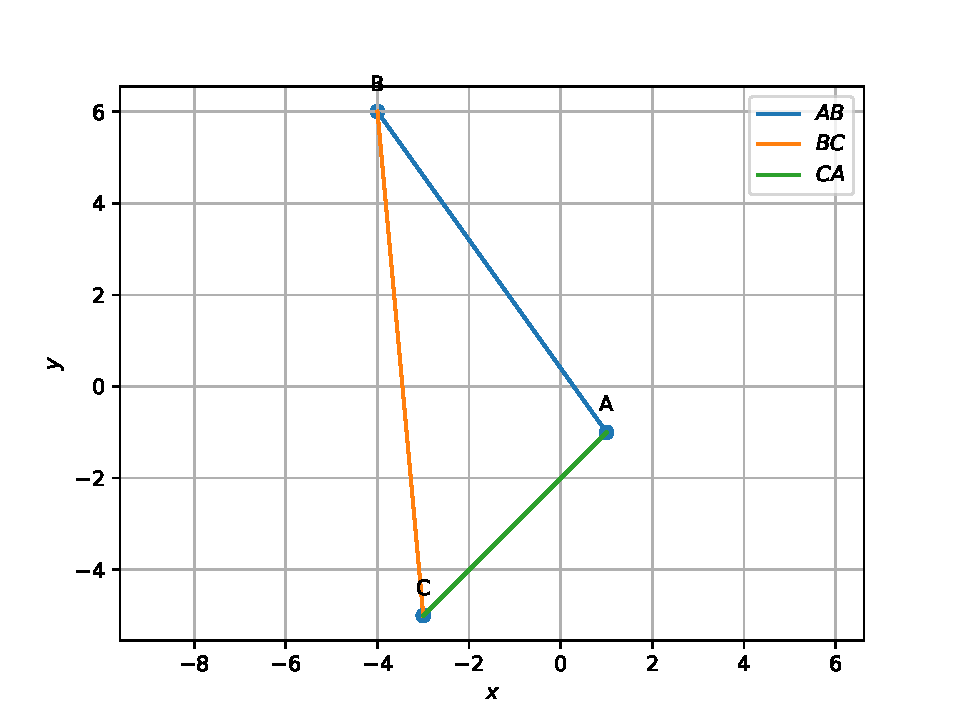
\includegraphics[width=\columnwidth]{figs/triangle/vector.pdf}
\caption{$\triangle ABC$}
\label{fig1:Triangle}
\end{figure}
% \\		\solution 
From 
			\eqref{eq:tri-pts},
\begin{align}
    \label{eq:1.1.3,2}
\myvec{
    1 & 1 & 1\\
    \vec{A} & \vec{B} & \vec{C} \\
    } 
    =
    %\label{eq:matthrowoperations}
    \myvec{
    1 & 1 & 1
    \\
    1 & -4 & -3
    \\
    -1 & 6 & -5
    }
     \xleftrightarrow[]{R_3 \leftarrow R_3+R_2}
    \myvec{
    1 & 1 & 1
    \\
    1 & -4 & -3
    \\
    0 & 2 & -8 
    }
    \\
     \xleftrightarrow[]{R_2\leftarrow R_1-R_2}
    \myvec{
    1 & 1 & 1
    \\
    0 & 5 & 4
    \\
    0 & 2 & -8 
    }
     \xleftrightarrow[]{R_3\leftarrow R_3-\frac{2}{5}R_2}
    \myvec{
    1 & 1 & 1
    \\
    0 & 5 & 4
    \\
    0 & 0 & \frac{-48}{5}
    }
\end{align}
There are no zero rows. So,
\begin{align}
    \text{rank}\myvec{
    1 & 1 & 1\\
    \vec{A} & \vec{B} & \vec{C} \\
    } &= 3 
\end{align}  
Hence,  the points $\vec{A},\vec{B},\vec{C}$ are not collinear. 
This is visible in 
\figref{fig1:Triangle}.
\begin{figure}[h]
\centering
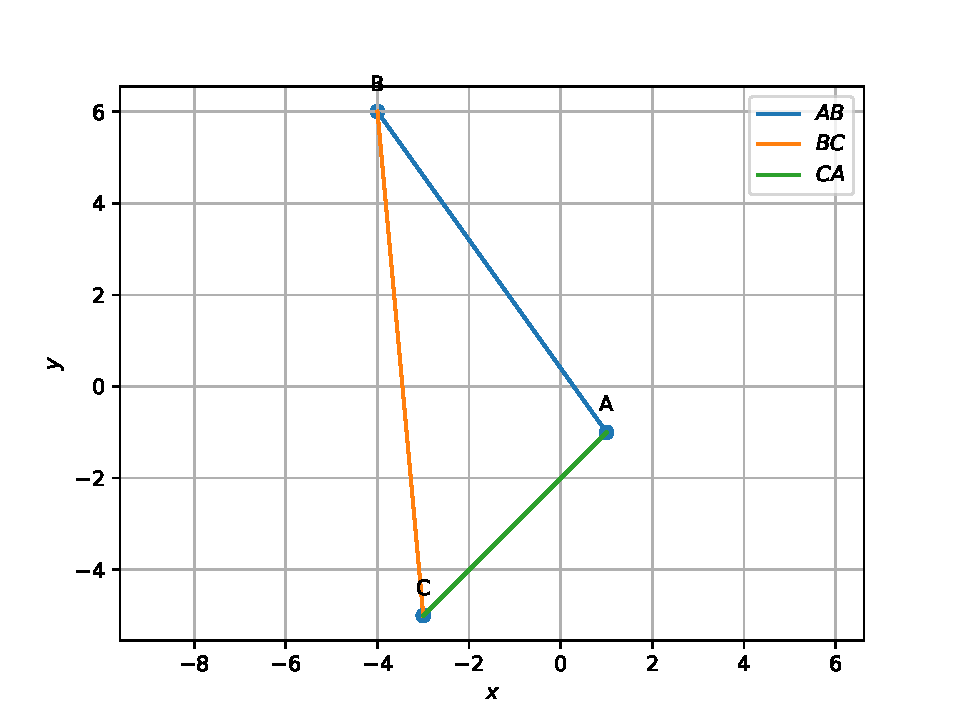
\includegraphics[width=\columnwidth]{figs/triangle/vector.pdf}
\caption{$\triangle ABC$}
\label{fig1:Triangle}
\end{figure}

\item The parameteric form of the equation  of $AB$ is 
		\begin{align}
			\label{eq:geo-param}
			\vec{x}=\vec{A}+k\vec{m} \quad k \ne 0,
		\end{align}
		where
		\begin{align}
\vec{m}=\vec{B}-\vec{A}
		\end{align}
is the direction vector of $AB$.
Find the parameteric equations of $AB, BC$ and $CA$.
\\
\solution
From 
			\eqref{eq:geo-param} and
		\eqref{eq:geo-dir-vec-ab},
the parametric equation for $AB$ is given by
\begin{align}
AB: \vec{x} = &\myvec{1\\-1} + k \myvec{-5\\7}
\end{align}
Similarly, from 
		\eqref{eq:geo-dir-vec-bc} and
		\eqref{eq:geo-dir-vec-ca},
\begin{align}
BC: \vec{x} = &\myvec{-4\\6} + k \myvec{1\\-11}\\
CA: \vec{x} = &\myvec{-3\\-5} + k \myvec{4\\4}
\end{align}

%		\solution
From 
			\eqref{eq:geo-param} and
		\eqref{eq:geo-dir-vec-ab},
the parametric equation for $AB$ is given by
\begin{align}
AB: \vec{x} = &\myvec{1\\-1} + k \myvec{-5\\7}
\end{align}
Similarly, from 
		\eqref{eq:geo-dir-vec-bc} and
		\eqref{eq:geo-dir-vec-ca},
\begin{align}
BC: \vec{x} = &\myvec{-4\\6} + k \myvec{1\\-11}\\
CA: \vec{x} = &\myvec{-3\\-5} + k \myvec{4\\4}
\end{align}


\item The normal form of the equation of $AB$  is 
		\begin{align}
			\label{eq:geo-normal}
			\vec{n}^{\top}\brak{	\vec{x}-\vec{A}} = 0
		\end{align}
		where 
		\begin{align}
			\vec{n}^{\top}\vec{m}&=\vec{n}^{\top}\brak{\vec{B}-\vec{A}} = 0
			\\
			\text{or, } \vec{n}&=\myvec{0 & 1 \\ -1 & 0} \vec{m}
			\label{eq:geo-norm-vec}
		\end{align}
Find the normal form of the equations of $AB, BC$ and $CA$.
\\
\solution
\begin{enumerate}
	\item
From
		\eqref{eq:geo-dir-vec-bc}, 
the direction vector of side $\vec{BC}$ is
\begin{align}
\vec{m}
	&=\myvec{1\\-11}
	\\
\implies \vec{n} &= \myvec{0 & 1\\
  -1 & 0}\myvec{1\\-11}
 = \myvec{-11\\-1}
		\label{eq:geo-norm-vec-bc}
\end{align}
from 
			\eqref{eq:geo-norm-vec}.
Hence, from 
			\eqref{eq:geo-normal},
the normal equation of side $BC$ is 
\begin{align}
	\vec{n}^{\top}\brak{	\vec{x}-\vec{B}} &= 0
			\\
\implies    \myvec{-11 & -1}\vec{x}&=\myvec{-11 & -1}\myvec{-4\\6}\\
    \implies
BC: \quad    \myvec{11 & 1}\vec{x}&=-38
\end{align}
\item Similarly, for $AB$,
from 
		\eqref{eq:geo-dir-vec-ab}, 
\begin{align}
	\vec{m} &= \myvec{-5\\7}
	\\
\implies        \vec{n} 
                &= \myvec{0&1\\-1&0}\myvec{-5\\7}
                = \myvec{7\\5}
		\label{eq:geo-norm-vec-ab}
\end{align}
and 
\begin{align}
	\vec{n}^{\top}\brak{	\vec{x}-\vec{A}} &= 0
	\\
	\implies
                AB: \quad  \vec{n}^{\top}\vec{x} &= \myvec{7&5}\myvec{1\\-1}\\    
       \implies\myvec{7&5}\vec{x} &= 2
\end{align}
\item For 
$CA$, 
from 
		\eqref{eq:geo-dir-vec-ca}, 
\begin{align}
\vec{m} &= \myvec{1 \\ 1}
\\
		\label{eq:geo-norm-vec-ca}
\implies \vec{n} 
&= \myvec{0&1 \\ -1&0}\myvec{1 \\ 1}
= \myvec{1 \\ -1}\\
\\
\implies	\vec{n}^{\top}\brak{	\vec{x}-\vec{C}} &= 0
\\
\implies \myvec{1&-1}{\vec{x}} &= \myvec{1&-1}\myvec{-3 \\ -5} 
= 2 
\end{align}
\end{enumerate}

%\begin{enumerate}
	\item
From
		\eqref{eq:geo-dir-vec-bc}, 
the direction vector of side $\vec{BC}$ is
\begin{align}
\vec{m}
	&=\myvec{1\\-11}
	\\
\implies \vec{n} &= \myvec{0 & 1\\
  -1 & 0}\myvec{1\\-11}
 = \myvec{-11\\-1}
		\label{eq:geo-norm-vec-bc}
\end{align}
from 
			\eqref{eq:geo-norm-vec}.
Hence, from 
			\eqref{eq:geo-normal},
the normal equation of side $BC$ is 
\begin{align}
	\vec{n}^{\top}\brak{	\vec{x}-\vec{B}} &= 0
			\\
\implies    \myvec{-11 & -1}\vec{x}&=\myvec{-11 & -1}\myvec{-4\\6}\\
    \implies
BC: \quad    \myvec{11 & 1}\vec{x}&=-38
\end{align}
\item Similarly, for $AB$,
from 
		\eqref{eq:geo-dir-vec-ab}, 
\begin{align}
	\vec{m} &= \myvec{-5\\7}
	\\
\implies        \vec{n} 
                &= \myvec{0&1\\-1&0}\myvec{-5\\7}
                = \myvec{7\\5}
		\label{eq:geo-norm-vec-ab}
\end{align}
and 
\begin{align}
	\vec{n}^{\top}\brak{	\vec{x}-\vec{A}} &= 0
	\\
	\implies
                AB: \quad  \vec{n}^{\top}\vec{x} &= \myvec{7&5}\myvec{1\\-1}\\    
       \implies\myvec{7&5}\vec{x} &= 2
\end{align}
\item For 
$CA$, 
from 
		\eqref{eq:geo-dir-vec-ca}, 
\begin{align}
\vec{m} &= \myvec{1 \\ 1}
\\
		\label{eq:geo-norm-vec-ca}
\implies \vec{n} 
&= \myvec{0&1 \\ -1&0}\myvec{1 \\ 1}
= \myvec{1 \\ -1}\\
\\
\implies	\vec{n}^{\top}\brak{	\vec{x}-\vec{C}} &= 0
\\
\implies \myvec{1&-1}{\vec{x}} &= \myvec{1&-1}\myvec{-3 \\ -5} 
= 2 
\end{align}
\end{enumerate}


\item The area of $\triangle ABC$ is defined as
		\begin{align}
			\label{eq:tri-area-cross}
			\frac{1}{2}\norm{{\brak{\vec{A}-\vec{B}}\times \brak{\vec{A}-\vec{C}}}}
		\end{align}
		where
		\begin{align}
			\vec{A}\times\vec{B} \triangleq \mydet{1 & -4 \\-1 & 6}
		\end{align}
		Find the area of $\triangle ABC$.\\
\solution
From
		\eqref{eq:geo-dir-vec-ab}
		and
		\eqref{eq:geo-dir-vec-ca},
\begin{align}
	\vec{A}-\vec{B}=\myvec{5\\-7},
	\vec{A}-\vec{C}&=\myvec{4\\4}\\
\implies (\vec{A}-\vec{B})\times(\vec{A}-\vec{C}) &=\mydet{5 & 4\\-7 & 4}\\
&=5\times 4-4\times (-7)\\&=48\\
\implies\frac{1}{2}\norm{(\vec{A}-\vec{B})\times(\vec{A}-\vec{C})}&=\frac{48}{2}=24
\end{align}
which is the desired area.

%  		\solution
From
		\eqref{eq:geo-dir-vec-ab}
		and
		\eqref{eq:geo-dir-vec-ca},
\begin{align}
	\vec{A}-\vec{B}=\myvec{5\\-7},
	\vec{A}-\vec{C}&=\myvec{4\\4}\\
\implies (\vec{A}-\vec{B})\times(\vec{A}-\vec{C}) &=\mydet{5 & 4\\-7 & 4}\\
&=5\times 4-4\times (-7)\\&=48\\
\implies\frac{1}{2}\norm{(\vec{A}-\vec{B})\times(\vec{A}-\vec{C})}&=\frac{48}{2}=24
\end{align}
which is the desired area.


	\item Find the angles $A, B, C$ if 
%    \label{prop:angle2d}
  \begin{align}
    \label{eq:angle2d}
			\cos A \triangleq 
\frac{\brak{\vec{B}-\vec{A}}^{\top}{\vec{C}-\vec{A}}}{\norm{\vec{B}-\vec{A}}\norm{\vec{C}-\vec{A}}}
  \end{align}\\
  \solution
\begin{enumerate}
	\item From 
		\eqref{eq:geo-dir-vec-ab},
		\eqref{eq:geo-dir-vec-ca},
		\eqref{eq:geo-norm-ab}
		and
		\eqref{eq:geo-norm-ca}
\begin{align}
	(\vec{B}-\vec{A})^{\top}(\vec{C}-\vec{A})&=\myvec{-5&7}\myvec{-4\\-4}\\
	&=-8
	\\
	\implies
	\cos{A}&= \frac{-8}{\sqrt{74} \sqrt{32}}
	= \frac{-1}{\sqrt{37}}\\
	\implies A&=\cos^{-1}{\frac{-1}{\sqrt{37}}}
\end{align}
	\item From 
		\eqref{eq:geo-dir-vec-ab},
		\eqref{eq:geo-dir-vec-bc},
		\eqref{eq:geo-norm-ab}
		and
		\eqref{eq:geo-norm-bc}
\begin{align}
	(\vec{C}-\vec{B})^{\top}(\vec{A}-\vec{B})&=\myvec{1&-11}\myvec{5\\-7}\\
	&= 82
	\\
	\implies
	\cos{B}&= \frac{82}{\sqrt{74} \sqrt{122}}
	= \frac{41}{\sqrt{2257}}\\
	\implies B&=\cos^{-1}{\frac{41}{\sqrt{2257}}}
\end{align}
	\item From 
		\eqref{eq:geo-dir-vec-bc},
		\eqref{eq:geo-dir-vec-ca},
		\eqref{eq:geo-norm-bc}
		and
		\eqref{eq:geo-norm-ca}
\begin{align}
	(\vec{A}-\vec{C})^{\top}(\vec{B}-\vec{C})&=\myvec{4&4}\myvec{-1\\11}\\
	&=40
	\\
\implies	\cos{C}&= \frac{40}{\sqrt{32} \sqrt{122}}
	= \frac{5}{\sqrt{61}}\\
	\implies C&=\cos^{-1}{\frac{5}{\sqrt{61}}}
\end{align}

\end{enumerate}
%  	\begin{enumerate}
	\item From 
		\eqref{eq:geo-dir-vec-ab},
		\eqref{eq:geo-dir-vec-ca},
		\eqref{eq:geo-norm-ab}
		and
		\eqref{eq:geo-norm-ca}
\begin{align}
	(\vec{B}-\vec{A})^{\top}(\vec{C}-\vec{A})&=\myvec{-5&7}\myvec{-4\\-4}\\
	&=-8
	\\
	\implies
	\cos{A}&= \frac{-8}{\sqrt{74} \sqrt{32}}
	= \frac{-1}{\sqrt{37}}\\
	\implies A&=\cos^{-1}{\frac{-1}{\sqrt{37}}}
\end{align}
	\item From 
		\eqref{eq:geo-dir-vec-ab},
		\eqref{eq:geo-dir-vec-bc},
		\eqref{eq:geo-norm-ab}
		and
		\eqref{eq:geo-norm-bc}
\begin{align}
	(\vec{C}-\vec{B})^{\top}(\vec{A}-\vec{B})&=\myvec{1&-11}\myvec{5\\-7}\\
	&= 82
	\\
	\implies
	\cos{B}&= \frac{82}{\sqrt{74} \sqrt{122}}
	= \frac{41}{\sqrt{2257}}\\
	\implies B&=\cos^{-1}{\frac{41}{\sqrt{2257}}}
\end{align}
	\item From 
		\eqref{eq:geo-dir-vec-bc},
		\eqref{eq:geo-dir-vec-ca},
		\eqref{eq:geo-norm-bc}
		and
		\eqref{eq:geo-norm-ca}
\begin{align}
	(\vec{A}-\vec{C})^{\top}(\vec{B}-\vec{C})&=\myvec{4&4}\myvec{-1\\11}\\
	&=40
	\\
\implies	\cos{C}&= \frac{40}{\sqrt{32} \sqrt{122}}
	= \frac{5}{\sqrt{61}}\\
	\implies C&=\cos^{-1}{\frac{5}{\sqrt{61}}}
\end{align}

\end{enumerate}

All codes for this section are available at
\begin{lstlisting}
	codes/triangle/sides.py
\end{lstlisting}
\end{enumerate}

\subsection{Median}
\begin{enumerate}[label=\thesubsection.\arabic*.,ref=\thesubsection.\theenumi]
\numberwithin{equation}{enumi}
\item If $\vec{D}$ divides $BC$ in the ratio $k : 1$,
		\begin{align}
			\vec{D}= \frac{k\vec{C}+\vec{B}}{k+1}
	  \label{eq:section_formula}
		\end{align}
		Find the mid points $\vec{D}, \vec{E}, \vec{F}$ of the sides $BC, CA$ and $AB$ respectively.
	\\
		\solution
Since $\vec{D}$ is the midpoint of $BC$,
\begin{align}
k &= 1,\\
\implies \vec{D} &= \frac{\vec{C} + \vec{B}}{2}
= \frac{1}{2}\myvec{-7\\1}
	\label{eq:median-d}
\end{align}
Similarly,
\begin{align}
	\label{eq:median-e}
\vec{E} &= \frac{\vec{A} + \vec{C}}{2}
= \myvec{-1\\-3}\\
\vec{F} &= \frac{\vec{A} + \vec{B}}{2}
= \frac{1}{2}\myvec{-3\\5}
	\label{eq:median-f}
\end{align}
  
	\item Find the equations of $AD, BE$ and $CF$.
	\\	\\ \solution:
\begin{enumerate}
 \item The direction vector of $AD$ is 
\begin{align}
	\vec{m} = \vec{D}- \vec{A}
&=\myvec{\frac{-7}{2}\\\frac{1}{2}} - \myvec{1\\-1}
	=\frac{1}{2}\myvec{-9\\3} \equiv \myvec{-3 \\ 1}
	\\
	\implies  \vec{n} &=\myvec{1 \\ 3}
\end{align}
Hence the normal equation of median $AD$ is 
\begin{align}
\vec{n}^{\top}\myvec{\vec{x}-\vec{A}}&=0\\
\implies    \myvec{1 & 3}\vec{x}&=\myvec{1 & 3}\myvec{1\\-1}
    =-2
	\label{eq:median-ad}
\end{align}
\item For $BE$,
\begin{align}
	\vec{m}= \vec{E}- \vec{B}&=\myvec{-1\\-3} - \myvec{-4\\6}
       =\myvec{3\\-9}
       \equiv \myvec{1\\-3}
       \\
\implies 	
\vec{n} &= 
         \myvec{3\\1}
\end{align}
Hence the normal equation of median $BE$ is 
\begin{align}
\vec{n}^{\top}\myvec{\vec{x}-\vec{B}}&=0\\
\implies
	\myvec{3 & 1}   \vec{x}&=\myvec{3 &1}\myvec{-4\\6}
    =-6
	\label{eq:median-be}
\end{align}
\item For median $CF$,
\begin{align}
	\vec{m} = \vec{F}- \vec{C} &=
\myvec{\frac{-3}{2}\\\frac{5}{2}} - \myvec{-3\\-5}
       =\myvec{\frac{3}{2}\\\frac{15}{2}}
       \equiv \myvec{1 \\ 5}
       \\
	\implies \vec{n} &=\myvec{5 \\ -1}
\end{align}
Hence the normal equation of median $CF$ is 
\begin{align}
\vec{n}^{\top}\myvec{\vec{x}-\vec{C}}&=0\\
	\implies \myvec{5 & -1}\vec{x}&=\myvec{5 & -1}\myvec{-3\\-5}
    =-10
	\label{eq:median-cf}
\end{align}
\end{enumerate}
\iffalse
\begin{figure}
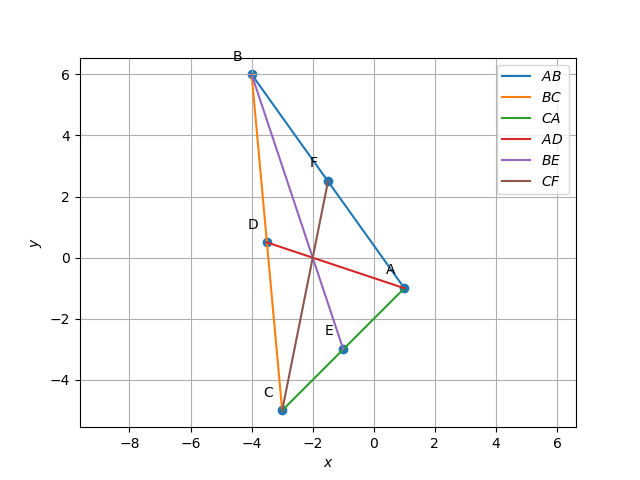
\includegraphics [width=\columnwidth] {solutions/1/2/2/figs/figure.png}
\caption{ Medians $AD$ , $BE$ and $CF$}
\label{fig: medians}
\end{figure}
\fi




% 		\iffalse
\let\negmedspace\undefined
\let\negthickspace\undefined
\documentclass[journal,12pt,twocolumn]{IEEEtran}
\usepackage{cite}
\usepackage{amsmath,amssymb,amsfonts,amsthm}
\usepackage{algorithmic}
\usepackage{graphicx}
\usepackage{textcomp}
\usepackage{xcolor}
\usepackage{txfonts}
\usepackage{listings}
\usepackage{enumitem}
\usepackage{mathtools}
\usepackage{gensymb}
\usepackage[breaklinks=true]{hyperref}
\usepackage{tkz-euclide} % loads  TikZ and tkz-base
\usepackage{listings}
\usepackage{gvv}
%
%\usepackage{setspace}
%\usepackage{gensymb}
%\doublespacing
%\singlespacing

%\usepackage{graphicx}
%\usepackage{amssymb}
%\usepackage{relsize}
%\usepackage[cmex10]{amsmath}
%\usepackage{amsthm}
%\interdisplaylinepenalty=2500
%\savesymbol{iint}
%\usepackage{txfonts}
%\restoresymbol{TXF}{iint}
%\usepackage{wasysym}
%\usepackage{amsthm}
%\usepackage{iithtlc}
%\usepackage{mathrsfs}
%\usepackage{txfonts}
%\usepackage{stfloats}
%\usepackage{bm}
%\usepackage{cite}
%\usepackage{cases}
%\usepackage{subfig}
%\usepackage{xtab}
%\usepackage{longtable}
%\usepackage{multirow}
%\usepackage{algorithm}
%\usepackage{algpseudocode}
%\usepackage{enumitem}
%\usepackage{mathtools}
%\usepackage{tikz}
%\usepackage{circuitikz}
%\usepackage{verbatim}
%\usepackage{tfrupee}
%\usepackage{stmaryrd}
%\usetkzobj{all}
%    \usepackage{color}                                            %%
%    \usepackage{array}                                            %%
%    \usepackage{longtable}                                        %%
%    \usepackage{calc}                                             %%
%    \usepackage{multirow}                                         %%
%    \usepackage{hhline}                                           %%
%    \usepackage{ifthen}                                           %%
  %optionally (for landscape tables embedded in another document): %%
%    \usepackage{lscape}     
%\usepackage{multicol}
%\usepackage{chngcntr}
%\usepackage{enumerate}

%\usepackage{wasysym}
%\documentclass[conference]{IEEEtran}
%\IEEEoverridecommandlockouts
% The preceding line is only needed to identify funding in the first footnote. If that is unneeded, please comment it out.

\newtheorem{theorem}{Theorem}[section]
\newtheorem{problem}{Problem}
\newtheorem{proposition}{Proposition}[section]
\newtheorem{lemma}{Lemma}[section]
\newtheorem{corollary}[theorem]{Corollary}
\newtheorem{example}{Example}[section]
\newtheorem{definition}[problem]{Definition}
%\newtheorem{thm}{Theorem}[section] 
%\newtheorem{defn}[thm]{Definition}
%\newtheorem{algorithm}{Algorithm}[section]
%\newtheorem{cor}{Corollary}
\newcommand{\BEQA}{\begin{eqnarray}}
\newcommand{\EEQA}{\end{eqnarray}}
\newcommand{\define}{\stackrel{\triangle}{=}}
\theoremstyle{remark}
\newtheorem{rem}{Remark}

%\bibliographystyle{ieeetr}
\begin{document}
%

\bibliographystyle{IEEEtran}


\vspace{3cm}

\title{ Solution of 1.2.2
%	\logo{

%	}
}
\author{ Dhruv Parashar$^{*}$% <-this % stops a space
	
}	
%\title{
%	\logo{Matrix Analysis through Octave}{\begin{center}\includegraphics[scale=.24]{tlc}\end{center}}{}{HAMDSP}
%}


% paper title
% can use linebreaks \\ within to get better formatting as desired
%\title{Matrix Analysis through Octave}
%
%
% author names and IEEE memberships
% note positions of commas and nonbreaking spaces ( ~ ) LaTeX will not break
% a structure at a ~ so this keeps an author's name from being broken across
% two lines.
% use \thanks{} to gain access to the first footnote area
% a separate \thanks must be used for each paragraph as LaTeX2e's \thanks
% was not built to handle multiple paragraphs
%

%\author{<-this % stops a space
%\thanks{}}
%}
% note the % following the last \IEEEmembership and also \thanks - 
% these prevent an unwanted space from occurring between the last author name
% and the end of the author line. i.e., if you had this:
% 
% \author{....lastname \thanks{...} \thanks{...} }
%                     ^------------^------------^----Do not want these spaces!
%
% a space would be appended to the last name and could cause every name on that
% line to be shifted left slightly. This is one of those "LaTeX things". For
% instance, "\textbf{A} \textbf{B}" will typeset as "A B" not "AB". To get
% "AB" then you have to do: "\textbf{A}\textbf{B}"
% \thanks is no different in this regard, so shield the last } of each \thanks
% that ends a line with a % and do not let a space in before the next \thanks.
% Spaces after \IEEEmembership other than the last one are OK (and needed) as
% you are supposed to have spaces between the names. For what it is worth,
% this is a minor point as most people would not even notice if the said evil
% space somehow managed to creep in.



% The paper headers
%\markboth{Journal of \LaTeX\ Class Files,~Vol.~6, No.~1, January~2007}%
%{Shell \MakeLowercase{\textit{et al.}}: Bare Demo of IEEEtran.cls for Journals}
% The only time the second header will appear is for the odd numbered pages
% after the title page when using the twoside option.
% 
% *** Note that you probably will NOT want to include the author's ***
% *** name in the headers of peer review papers.                   ***
% You can use \ifCLASSOPTIONpeerreview for conditional compilation here if
% you desire.




% If you want to put a publisher's ID mark on the page you can do it like
% this:
%\IEEEpubid{0000--0000/00\$00.00~\copyright~2007 IEEE}
% Remember, if you use this you must call \IEEEpubidadjcol in the second
% column for its text to clear the IEEEpubid mark.



% make the title area
\maketitle

\newpage

%\tableofcontents

\bigskip

\renewcommand{\thefigure}{\theenumi}
\renewcommand{\thetable}{\theenumi}
%\renewcommand{\theequation}{\theenumi}

%\begin{abstract}
%%\boldmath
%In this letter, an algorithm for evaluating the exact analytical bit error rate  (BER)  for the piecewise linear (PL) combiner for  multiple relays is presented. Previous results were available only for upto three relays. The algorithm is unique in the sense that  the actual mathematical expressions, that are prohibitively large, need not be explicitly obtained. The diversity gain due to multiple relays is shown through plots of the analytical BER, well supported by simulations. 
%
%\end{abstract}
% IEEEtran.cls defaults to using nonbold math in the Abstract.
% This preserves the distinction between vectors and scalars. However,
% if the journal you are submitting to favors bold math in the abstract,
% then you can use LaTeX's standard command \boldmath at the very start
% of the abstract to achieve this. Many IEEE journals frown on math
% in the abstract anyway.

% Note that keywords are not normally used for peerreview papers.
%\begin{IEEEkeywords}
%Cooperative diversity, decode and forward, piecewise linear
%\end{IEEEkeywords}



% For peer review papers, you can put extra information on the cover
% page as needed:
% \ifCLASSOPTIONpeerreview
% \begin{center} \bfseries EDICS Category: 3-BBND \end{center}
% \fi
%
% For peerreview papers, this IEEEtran command inserts a page break and
% creates the second title. It will be ignored for other modes.
%\IEEEpeerreviewmaketitle


Question:- 
We are given the three vertices of a triangle$(A,B,C)$ and the midpoints $\vec{D},\vec{E},\vec{F}$ of the sides $AB,BC,AC$ respectively. We have to find the equations of the sides $AD,BE,CF$.
\\
\fi
\solution
\begin{align}
\vec{A} &= \myvec{1\\-1} \\
\vec{B} &= \myvec{-4\\6} \\
\vec{C} &= \myvec{-3\\-5}
\end{align}
The mid points $\vec{D},\vec{E},\vec{F}$ of sides $AB,BC,AC$ are :-
\begin{align}
\vec{D} &= \frac{1}{2}\myvec{-7  \\ 1}\\
\vec{E} &= \myvec{-1\\-3}\\
\vec{F} &= \frac{1}{2}\myvec{-3  \\ 5}
\end{align}
Now, the direction vector of line $FC(\vec{m})$ is :-
\begin{align}
\vec{m} &= \vec{F} - \vec{C} \\
\implies \vec{m} &= \frac{1}{2}\myvec{3 \\ 15}
\end{align}
Now, we have to find $\vec{n}$,
\begin{align}
\vec{n} &= \myvec{0 & 1 \\ -1 & 0}\vec{m}\\
&= \frac{1}{2}\myvec{0 & 1 \\ -1 & 0}\myvec{3\\15}\\
&=\frac{1}{2}\myvec{15\\-3}
\end{align}
Normal form of line CF is :
\begin{align}
\vec{n}^{\top}(\vec{x-C}) &= 0\\
\vec{n}^{\top}\vec{x} &= \vec{n}^{\top}\vec{C} \\
\frac{1}{2}\myvec{15 & -3}\vec{x} &= \frac{1}{2}\myvec{15 & -3}\myvec{-3\\-5} \\
\myvec{15 & -3}\vec{x} &= \myvec{15 & -3}\myvec{-3\\-5} \\
\myvec{15 & -3}\vec{x} &= -30
\end{align}

\begin{figure}
\centering
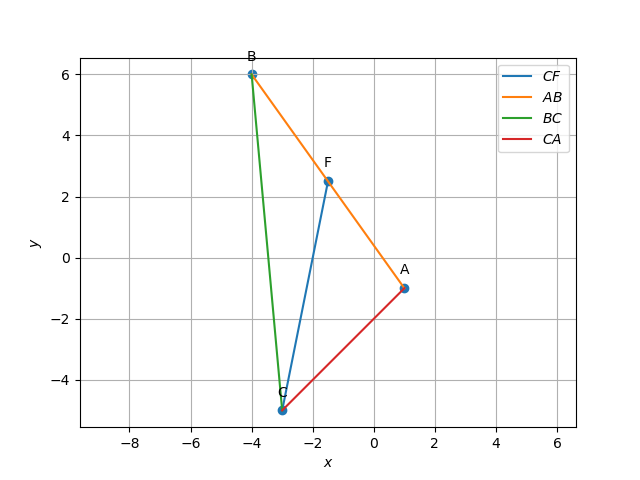
\includegraphics[width=\columnwidth]{solutions/1/2/2a/figs/figure.png}
\caption{Line CF}
\label{fig:Line CF}
\end{figure}



	\item Find the intersection $\vec{G}$ of $BE$ and $CF$.
 \\
\solution 
From 
	\eqref{eq:median-be}
	and
	\eqref{eq:median-cf},
the equations of $BE$ 
and 
$CF$
are, respectively,
\begin{align}
\myvec{3 & 1} \vec{x} &= \myvec{-6}
\label{eq:1.2.3,8}
\\
\myvec{ 5&-1} \vec{x} &= \myvec{-10}
\label{eq:1.2.3,9}
\end{align}
From \eqref{eq:1.2.3,8} and \eqref{eq:1.2.3,9} the augmented matrix is
\begin{align}
    \label{eq:matrowoperations}
    \myvec{
    3 & 1 & -6
    \\
    5 & -1 & -10
    }
     \xleftrightarrow[]{R_1 \leftarrow R_1+R_2}
    \myvec{
    8 & 0 & -16
    \\
    5 & -1 & -10 
    }
    \\
     \xleftrightarrow[]{R_1\leftarrow R_1/8}
    \myvec{
    1 & 0 & -2
    \\
    5 & -1 & -10 
    }
     \xleftrightarrow[]{R_2\leftarrow R_2-5R_1}
    \myvec{
    1 & 0 & -2
    \\
    0 & -1 & 0
    }
    \\
     \xleftrightarrow[]{R_2\leftarrow -R_2}
    \myvec{
    1 & 0 & -2
    \\
    0 & 1 & 0
    }
\end{align} 
using Gauss elimination.  Therefore, 
\begin{align}
\vec{G} = \myvec{-2 \\ 0}
	\label{eq:median-g}
\end{align}

	\item Verify that 
		\begin{align}
			\frac{BG}{GE} = 
			\frac{CG}{GF} =
			\frac{AG}{GD} =2 
		\end{align}
		\\	\solution 
\begin{enumerate}
\item From 
	\eqref{eq:median-e}
	and
	\eqref{eq:median-g},
\begin{align}
		\label{eq:tri-pts/4} \vec{G}-\vec{B} &= \myvec{2 \\ -6},\, 
 \vec{E}-\vec{G} = \myvec{1 \\ -3} \\
	\implies \vec{G}-\vec{B} &= 2 \brak{ \vec{E}-\vec{G} }
	\\
	\implies \norm{\vec{G}-\vec{B}} &= 2 \norm{ \vec{E}-\vec{G} }
	\\
	\text{or, }		\label{eq:tri-pts/8}\frac{BG}{GE} &=  2  
\end{align}		
\item From 
	\eqref{eq:median-f}
	and
	\eqref{eq:median-g},
\begin{align}
		 \vec{F}-\vec{G} &= \frac{1}{2}\myvec{ 1 \\ 5},\, 
 \vec{G}-\vec{C} &= \myvec{1 \\ 5} \\
	\implies 		 \vec{G}-\vec{C} &= 2 \brak{\vec{F}-\vec{G}} 
	\\
	\implies 		 \norm{\vec{G}-\vec{C}} &= 2 \norm{\vec{F}-\vec{G}} 
	\\
		\text{or, }	\frac{CG}{GF} &=  2		
\label{eq:tri-pts/9}
\end{align}
\item From
	\eqref{eq:median-d}
	and
	\eqref{eq:median-g},
\begin{align}
		\label{eq:tri-pts/14} \vec{G}-\vec{A} &= \myvec{-3 \\ 1} ,\,
 \vec{D}-\vec{G} = \frac{1}{2}\myvec{ -3 \\ 1}
 \\
	\vec{G}-\vec{A} &= 
	2\brak{ \vec{D}-\vec{G} } 
	\\
\implies		 \norm{\vec{G}-\vec{A}} &= 
 2\norm{\vec{D}-\vec{G}} 
 \\
		\text{or, }		\label{eq:tri-pts/18}\frac{AG}{GD} &=   2		
\end{align}
\end{enumerate}
From \eqref{eq:tri-pts/8}, \eqref{eq:tri-pts/9}, \eqref{eq:tri-pts/18}
\begin{align}
		\frac{BG}{GE} = 
		\frac{CG}{GF} =
		\frac{AG}{GD} = 2
\end{align}

	\item Show that $\vec{A}, \vec{G}$ and $\vec{D}$ are collinear.
	\\
		\solution 
Points $\vec{A},\vec{D},\vec{G}$ are defined to be collinear if 
\begin{align}
    \text{rank}\myvec{
    1 & 1 & 1\\
    \vec{A} & \vec{D} & \vec{G} \\
    } = 2 
    \label{eq:mat_row_operations}
    \\
\implies    
    \myvec{
    1 & 1 & 1
    \\
    1 & -\frac{7}{2} & -2
    \\
    -1 & \frac{1}{2} & 0
    }
     \xleftrightarrow[]{R_3 \leftarrow R_3+R_2}
    \myvec{
    1 & 1 & 1
    \\
    1 & -\frac{7}{2} & -2
    \\
    0 & -3 & -2 
    }
    \\
     \xleftrightarrow[]{R_2\leftarrow R_2-R_1}
    \myvec{
    1 & 1 & 1
    \\
    0 & -\frac{9}{2} & -3
    \\
    0 & -3 & -2 
    }
     \xleftrightarrow[]{R_3\leftarrow R_3-\frac{2}{3}R_2}
    \myvec{
    1 & 1 & 1
    \\
    0 & -\frac{9}{2} & -3
    \\
    0 & 0 & 0
    }
\end{align}
Thus, the matrix 
    \eqref{eq:mat_row_operations}
    has rank 2 and the points are collinear.
    Thus, the medians of a triangle meet at the point $\vec{G}$.
See \figref{fig:Triangle-median}.
\begin{figure}
\centering
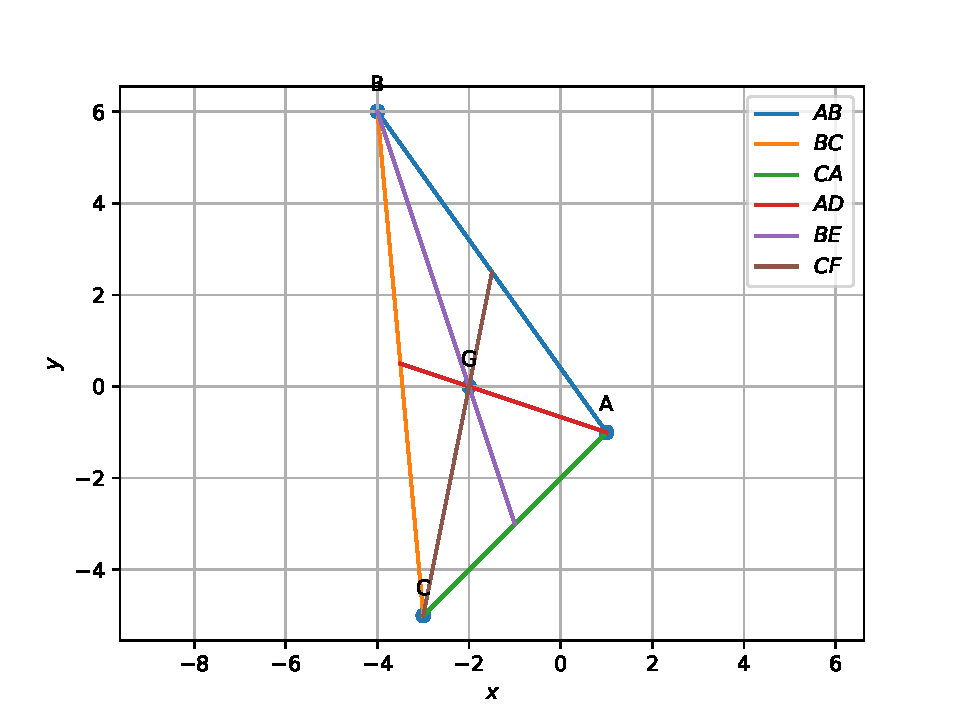
\includegraphics[width=\columnwidth]{figs/triangle/median.pdf}
	\caption{Medians of $\triangle ABC$ meet at $\vec{G}$.}
\label{fig:Triangle-median}
\end{figure}


	\item Verify that 
		\begin{align}
			\vec{G}=\frac{\vec{A}+\vec{B}+\vec{C}}{3}
		\end{align}
			$\vec{G}$ is known as the {\em centroid} of $\triangle ABC$.
   \\
		\solution
\begin{equation}
\begin{split}
\label{eq:centroid}
    \vec{G}&= \frac{\myvec{1\\-1}+\myvec{-4\\6}+\myvec{-3\\-5}}{3}\\    
     &= \myvec{-2\\0}
\end{split}
\end{equation}

 




	\item Verify that 
		\begin{align}
\vec{A}-\vec{F}=\vec{E}-\vec{D}
		\end{align}
		The quadrilateral $AFDE$ is defined to be a parallelogram.\\
  		\\ \solution 
\begin{align}
    \vec{A}-\vec{F}&=\myvec{1\\-1}-\myvec{\frac{-3}{2}\\\frac{5}{2}}
    =\myvec{\frac{5}{2}\\\frac{-7}{2}}
    \\
    \vec{E}-\vec{D}&=\myvec{-1\\-3}-\myvec{\frac{-7}{2}\\\frac{1}{2}}
    =\myvec{\frac{5}{2}\\\frac{-7}{2}}
    \\
	\implies	\vec{A}-\vec{F} &= \vec{E}-\vec{D}
\end{align}
See \figref{fig:Triangle-pgm}, 
\begin{figure}
\centering
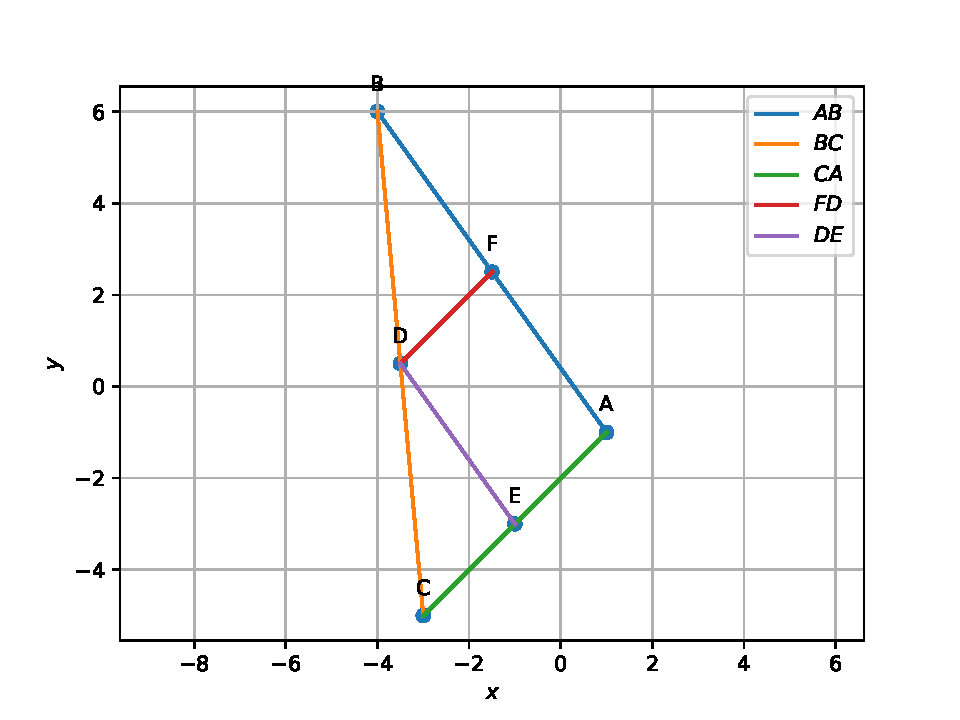
\includegraphics[width=\columnwidth]{figs/triangle/pgm.pdf}
\caption{$AFDE$ forms a parallelogram in triangle ABC}
\label{fig:Triangle-pgm}
\end{figure}






















All codes for this section are available in 
\begin{lstlisting}
	codes/triangle/medians.py
	codes/triangle/pgm.py
\end{lstlisting}
  
\end{enumerate}

\subsection{Altitude}
\begin{enumerate}[label=\thesubsection.\arabic*.,ref=\thesubsection.\theenumi]
\numberwithin{equation}{enumi}
\numberwithin{figure}{enumi}
\item $\vec{D}_1$ is a point on $BC$ such that
		\begin{align}
			AD_1 \perp BC
		\end{align}
		and $AD_1$ is defined to be the altitude. 
		Find the normal vector of $AD_1$.
  \\
		\solution
The normal vector of $AD_{1}$ 
is
the direction vector $BC$ and is obtained from  
		\eqref{eq:geo-dir-vec-bc}
		as
\begin{align}
	\vec{n} = 
\myvec{1\\-11}
\end{align}


	\item Find the equation of $AD_1$.
 \\     \solution
The equation of $AD_1$ is
\begin{align}
 \vec{n}^{\top}(\vec{x-A}) &= 0 \\
\implies \myvec{-1 & 11}\vec{x} &= \myvec{-1 & 11}\myvec{1 \\ -1}
= -12
\end{align}


	\item Find the equations of the altitudes $BE_1$ and $CF_1$ to the sides $AC$ and $AB$ respectively. 
  \\     \\ \solution
\begin{enumerate}
\item 
	From 
		\eqref{eq:geo-dir-vec-ca},
the normal vector of $CF_1$ is 
\begin{align}
\vec{n}&=\myvec{-5\\7} 
\end{align}
and the equation of $CF_1$ is
\begin{align}
\vec{n}^{\top}\brak{\vec{x}-\vec{C}}&=0 \\
\implies 
\myvec{-5 & 7}\brak{\vec{x}-\myvec{-3\\-5}}&=0  \\
	\implies \myvec{5 & -7}\vec{x}&=20
		\label{eq:geo-alt-cf},
\end{align}
\item Similarly, 
	from 
		\eqref{eq:geo-dir-vec-ab},
the normal vector of $BE_1$ is 
\begin{align}
\vec{n}= \myvec{1 \\1}
\end{align}
and the equation of  $BE_1$ is
\begin{align}
\vec{n}^{\top}\brak{\vec{x}-\vec{B}}&=0 \\
	\implies \myvec{1 & 1}\brak{\vec{x}-\myvec{-4\\6}}&=0 \\
	\implies \myvec{1 & 1}\vec{x}&=2
		\label{eq:geo-alt-be},
\end{align}
\end{enumerate}



	\item Find the intersection $\vec{H}$ of $BE_1$ and $CF_1$.
 \\
        \\ \solution
%
The intersection of 
		\eqref{eq:app-geo-alt-be}
		and
		\eqref{eq:app-geo-alt-cf},
		is obtained from 
		the matrix equation
		%
\begin{align}
        \myvec{1&1\\5&-7} \vec{x} &= \myvec{2\\20}
\end{align}
%
which can be solved as 
%
\begin{align}
        \myvec{1&1&2\\5&-7&20}
	 \xleftrightarrow[]{R_2 \leftarrow R_2 - 5R_1}
        \myvec{1&1&2\\0&-12&10}\\
	 \xleftrightarrow[]{R_2 \leftarrow \frac{R_2}{-12}}
        \myvec{1&1&2\\0&1&\frac{-5}{6}}
	 \xleftrightarrow[]{R_1 \leftarrow R_1 - R_2}
        \myvec{1&0&\frac{17}{6}\\0&1&\frac{-5}{6}}
\end{align}
%
yielding
%
\begin{align}
        \vec{H}&=\frac{1}{6}\myvec{{17}\\-{5}}
		\label{eq:app-geo-alt-H},
\end{align}
%
See 
\figref{fig:m_tri_py}
\begin{figure}[H]
\centering
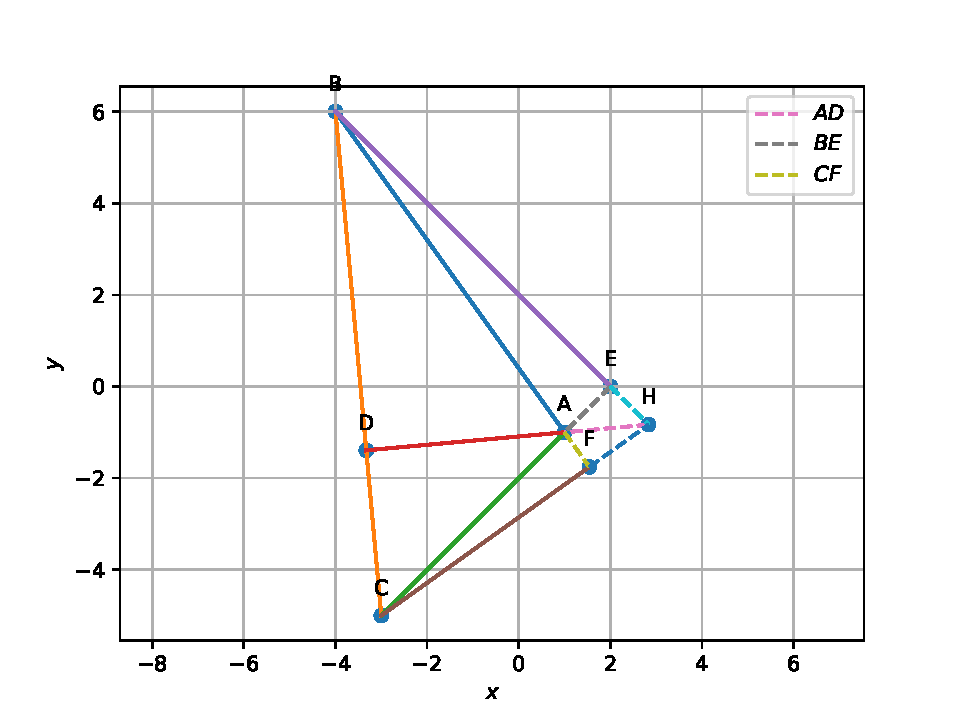
\includegraphics[width=0.75\columnwidth]{figs/triangle/altitude.pdf}
\caption{Altitudes $BE_1$ and $CF_1$ intersect at $\vec{H}$}
\label{fig:m_tri_py}
\end{figure}


	\item Verify that 
		\begin{align}
			\brak{\vec{A}-\vec{H}}^{\top}\brak{\vec{B}-\vec{C}} = 0
		\end{align}
  \solution
From 
		\eqref{eq:geo-alt-H},
\begin{align}
\vec{A}-\vec{H}=-\frac{1}{6}\myvec{{11}\\{1}},\,
\vec{B}-\vec{C}=\myvec{-1\\11}
\\
	\implies \brak{\vec{A}-\vec{H}}^{\top}\brak{\vec{B}-\vec{C}}=\frac{1}{6}\myvec{11 & 1}
\myvec{-1\\11}
=0
\end{align}


All codes for this section are available at
\begin{lstlisting}
	codes/triangle/altitude.py
\end{lstlisting}
\end{enumerate}

\subsection{Perpendicular Bisector}
\begin{enumerate}[label=\thesubsection.\arabic*.,ref=\thesubsection.\theenumi]
\numberwithin{equation}{enumi}

\item The equation of the perpendicular bisector of $BC$ is
		\begin{align}
			\label{eq:tri-perp-bisect}
			\brak{\vec{x}-\frac{\vec{B}+\vec{C}}{2}}\brak{\vec{B}-\vec{C}} = 0
		\end{align}
		Substitute numerical values and find the equations of the perpendicular bisectors of $AB, BC$ and $CA$.
	\\	\solution
From 
		\eqref{eq:app-geo-dir-vec-ab},
		\eqref{eq:app-geo-dir-vec-bc},
		\eqref{eq:app-geo-dir-vec-ca},
	\eqref{eq:median-d},
	\eqref{eq:median-e}
	and
	\eqref{eq:median-f},
\begin{align}
\vec{\frac{\vec{B}+\vec{C}}{2}} &= \frac{1}{2}\myvec{-{7} \\ 1},\,
\vec{B}-\vec{C} = \myvec{-1 \\ 11} 
\\
\vec{\frac{\vec{A}+\vec{B}}{2}}&=\frac{1}{2}\myvec{-{3} \\{5}},\,
\vec{A}-\vec{B}=\myvec{5\\ -7} \\
\vec{\frac{\vec{C}+\vec{A}}{2}} &= \myvec{-1\\-3},\,
\vec{C}-\vec{A} = \myvec{-4\\-4} 
\end{align}
yielding
\begin{alignat}{2}
  \brak{\vec{B}-\vec{C}}^{\top}\brak{\frac{\vec{B}+\vec{C}}{2}}
	&=\myvec{-1&11}\myvec{-\frac{7}{2} \\ \frac{1}{2}}
	&&=9
  \\
\brak{\vec{A}-\vec{B}}^{\top}\brak{\frac{\vec{A}+\vec{B}}{2}}
	&=\myvec{5&-7}\myvec{-\frac{3}{2} \\\frac{5}{2}}
	&&=-25
  \\
\brak{\vec{C}-\vec{A}}^{\top}\brak{\frac{\vec{C}+\vec{A}}{2}}
	&=\myvec{-4&-4}\myvec{-1\\-3}
	&&=16
\end{alignat}
Thus, the perpendicular bisectors are obtained from 
			\eqref{eq:tri-perp-bisect}
			as
		\begin{alignat}{2}
			\label{eq:app-tri-perp-bisect-bc}
			BC&: \quad \myvec{-1&11}\vec{x}&&=9
\\
			\label{eq:app-tri-perp-bisect-ca}
			CA&: \quad \myvec{5&-7}\vec{x}&&=-25
\\
			\label{eq:app-tri-perp-bisect-ab}
			AB&: \quad \myvec{1&1}\vec{x}&&=-4
		\end{alignat}




	\item Find the intersection $\vec{O}$ of the perpendicular bisectors of $AB$ and $AC$.
 \\
 \solution \\
The intersection of 
			\eqref{eq:app-tri-perp-bisect-ca}
			and
			\eqref{eq:app-tri-perp-bisect-ab},
			can be obtained as
\begin{align}
\myvec{5&-7&-25\\1&1&-4} \xleftrightarrow[]{R_2 \leftarrow 5R_2 - R_1} \myvec{5&-7&-25\\0&12&5}\\
 \xleftrightarrow[]{R_1\leftarrow \frac{12}{7}R_1 + R_2} \myvec{\frac{60}{7}&0& \frac{-265}{7}\\0&12&5}
 \xleftrightarrow[R_1\leftarrow \frac{7}{60}R_1]{R_2 \leftarrow \frac{1}{12}R_2} \myvec{1&0& \frac{-53}{12}\\0&1&\frac{5}{12}}\\
\implies \vec{O}=\myvec{\frac{-53}{12}\\\frac{5}{12}}
			\label{eq:app-tri-perp-bisect-O}
\end{align}

	\item Verify that $\vec{O}$ satisfies
			\eqref{eq:tri-perp-bisect}.
$\vec{O}$ is known as the circumcentre.\\
    \solution
Substituing  from 
			\eqref{eq:tri-perp-bisect-O} in 
			\eqref{eq:tri-perp-bisect},
when substituted in the above equation,
\begin{multline}
	\brak{\vec{O}-\frac{\vec{B}+\vec{C}}{2}}^{\top}\brak{\vec{B}-\vec{C}}\\
	=\brak{\frac{1}{12}\myvec{-53\\5}- \frac{1}{2}\myvec{-7\\1}}^{\top} \myvec{-1\\11}\\
	=\frac{1}{12}\myvec{-11&-1}\myvec{-1\\11}
	=0
\end{multline}




		\item Verify that 
		\begin{align}
			OA = OB = OC 
		\end{align}
	\item Draw the circle with centre at $\vec{O}$ and radius 
		\begin{align}
			R = OA
		\end{align}
		This is known as the {\em circumradius}. 
  \\  \solution 
See 
\figref{fig:circumcircle with centre O}.
\begin{figure}
\centering
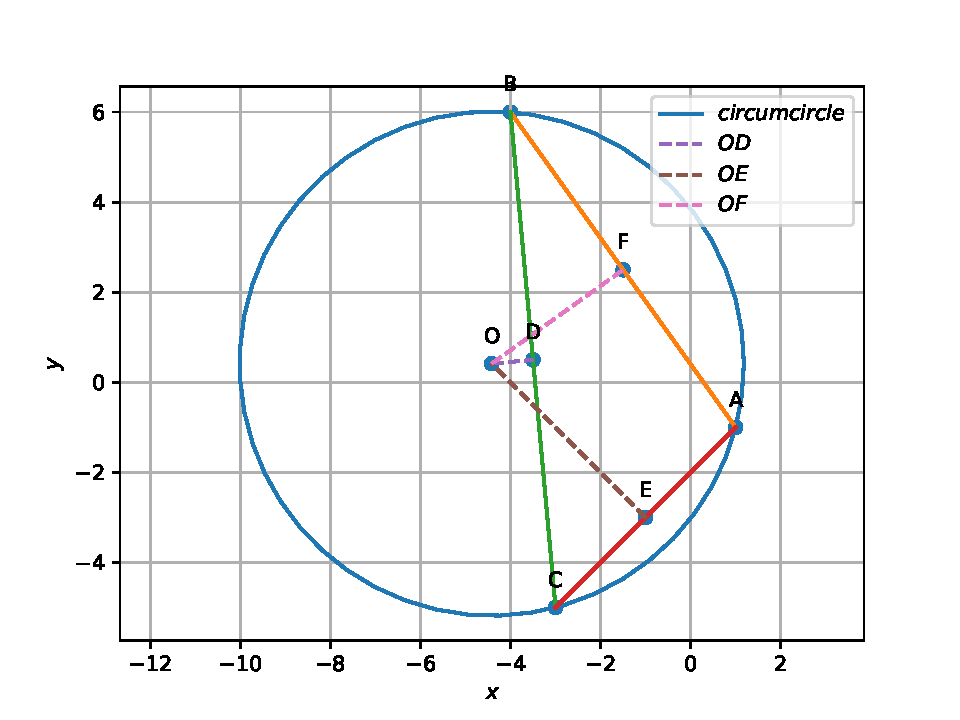
\includegraphics[width=0.75\columnwidth]{figs/triangle/perp-bisect.pdf}
	\caption{Circumcircle of $\triangle ABC$ with centre $\vec{O}$.}
\label{fig:circumcircle with centre O}	
\end{figure}


	\item Verify that 
		\begin{align}
			\angle BOC = 2\angle BAC.
		\end{align}\\
  \solution
\begin{enumerate}
\item To find  the value of $\angle{BOC}$ :
\begin{align}
\vec{B}-\vec{O}
          &=\myvec{\frac{5}{12}\\\frac{67}{12}},\,
\vec{C}-\vec{O}
          =\myvec{\frac{17}{12}\\\frac{-65}{12}}
	  \\
\implies \brak{\vec{B}-\vec{O}}^{\top}\brak{\vec{C}-\vec{O}}&=\frac{-4270}{144}\\
	\implies \norm{\vec{B}-\vec{O}}&= \frac{\sqrt{4514}}{12},\,
	\norm{\vec{C}-\vec{O}}= \frac{\sqrt{4514}}{12}
\end{align}
Thus,
\begin{align}
\cos{BOC}&=\frac{\brak{\vec{B}-\vec{O}}^{\top}\brak{\vec{C}-\vec{O}}}{\norm{\vec{B}-\vec{O}}\norm{\vec{C}-\vec{O}}}
=\frac{-4270}{4514}\\
\implies\angle{BOC}&=\cos^{-1}\brak{\frac{-4270}{4514}}
\\
	&=161.07536\degree
	\text{ or }
	198.92464\degree\label{eq:1}
\end{align}
	\item To find  the value of $\angle{BAC}$ :
\begin{align}
\vec{B}-\vec{A}&=\myvec{-5\\7},\,
\vec{C}-\vec{A}=\myvec{-4\\-4}
\\
\implies \brak{\vec{B}-\vec{A}}^{\top}\brak{\vec{C}-\vec{A}}&=-8
\\
	\norm{\vec{B}-\vec{A}}&= \sqrt{74}
	\norm{\vec{C}-\vec{A}}= 4\sqrt{2}
\end{align}
Thus,
\begin{align}
\cos{BAC}&=\frac{\brak{\vec{B}-\vec{A}}^{\top}\brak{\vec{C}-\vec{A}}}{\norm{\vec{B}-\vec{A}}\norm{\vec{C}-\vec{A}}}
=\frac{-8}{4\sqrt{148}}\\
\implies\angle{BAC}&=\cos^{-1}\brak{\frac{-8}{4\sqrt{148}}}\\
&=99.46232\degree \label{eq:2}
\end{align}
From \eqref{eq:2} and \eqref{eq:1},
\begin{align}
2\times\angle{BAC}
= \angle{BOC}
\end{align}
\end{enumerate}





	\item Let 
		\begin{align}
			\vec{P} = \myvec{\cos \theta & -\sin \theta \\ \sin \theta & \cos \theta}
		\end{align}
			where
\begin{align}
	\theta = \angle BOC
\end{align}
Verify that 
		\begin{align}
			\vec{B}-\vec{O}=\vec{P}\brak{\vec{C}-\vec{O}}
		\end{align}
All codes for this section are available at
\begin{lstlisting}
	codes/triangle/perp-bisect.py
\end{lstlisting}
\end{enumerate}

\subsection{Angle Bisector}
\begin{enumerate}[label=\thesubsection.\arabic*.,ref=\thesubsection.\theenumi]
\numberwithin{equation}{enumi}
\numberwithin{figure}{enumi}
	\item Let $\vec{D}_3, \vec{E}_3, \vec{F}_3$, be points on $AB, BC$ and $CA$ respectively such that
		\begin{align}
			BD_3 = BF_3=m, CD_3 = CE_3=n, AE_3 = AF_3=p.
		\end{align}
	Obtain $m,n,p$ in terms of $a,b,c$ obtained in  
		\probref{prob:side-length}.
 \\
 		\solution 
From the given information, 
\begin{align}
% 
    a &= m+n,\\
    b &= n+p, \\
    c &= m+p 
\end{align}
which can be expressed as
\begin{align}
\myvec{1&1&0\\0&1&1\\1&0&1\\}\myvec{m\\n\\p} &= \myvec{a\\b\\c}
\\
\implies 
	\myvec{m\\n\\p} &= \myvec{1&1&0\\0&1&1\\1&0&1\\}^{-1}\myvec{a\\b\\c}
\end{align}
Using row reduction,
		\begin{align}
			\augvec{3}{3}{1&1&0 & 1 & 0 & 0\\0&1&1 & 0 & 1 & 0\\1&0&1 & 0 & 0 & 1}
			\\
			\xleftrightarrow[]{R_3 \leftarrow R_3 - R_1}
			\augvec{3}{3}{1&1&0 & 1 & 0 & 0\\0&1&1 & 0 & 1 & 0\\0&-1&1 & -1 & 0 & 1}
			\\
			\xleftrightarrow[R_1 \leftarrow R_1 - R_2]{R_3 \leftarrow R_3 + R_2}
			\augvec{3}{3}{1&0&-1 & 1 & -1 & 0\\0&1&1 & 0 & 1 & 0\\0&0&2 & -1 & 1 & 1}
		\end{align}
		\begin{align}
			\xleftrightarrow[R_1 \leftarrow 2R_1 + R_3]{R_2 \leftarrow 2R_2 - R_3}
			\augvec{3}{3}{2&0&0 & 1 & -1 & 1\\0&2&0 & 1 & 1 & -1\\0&0&2 & -1 & 1 & 1}
		\end{align}
yielding
		\begin{align}
			\myvec{1&1&0\\0&1&1\\1&0&1\\}^{-1} = 
			\frac{1}{2}\myvec{1 & -1 & 1\\ 1 & 1 & -1\\ -1 & 1 & 1}
		\end{align}
	Therefore,
\begin{align}
\begin{split}
    p&=\frac{c+b-a}{2}
    =\frac{\sqrt{74}+\sqrt{32}-\sqrt{122}}{2}
    \\
    m&=\frac{a+c-b}{2}
    =\frac{\sqrt{74}+\sqrt{122}-\sqrt{32}}{2}
    \\
    n&=\frac{a+b-c}{2}
    =\frac{\sqrt{122}+\sqrt{32}-\sqrt{74}}{2}
\end{split}
	\label{eq:incircle-mnp}
\end{align}
upon substituting from 
		\eqref{eq:geo-norm-ab},
		\eqref{eq:geo-norm-bc}
		and
		\eqref{eq:geo-norm-ca}.

	\item Using section formula, find 
		\begin{align}
			\vec{D}_3 = \frac{m\vec{C}+n\vec{B}}{m+n},\,
			\vec{E}_3 = \frac{n\vec{A}+p\vec{C}}{n+p},\,
			\vec{F}_3 = \frac{p\vec{B}+m\vec{A}}{p+m}
		\end{align}
	\item Find the circumcentre and circumradius of $\triangle D_3E_3F_3$.  These are the {\em incentre} and {\em inradius} of $\triangle ABC$.
	\item Draw the circumcircle of $\triangle D_3E_3F_3$.  This is known as the {\em incircle} of $\triangle ABC$.
		\\
 		\solution
See 
	\figref{fig:incircle}
\begin{figure}[!ht]
	\centering
	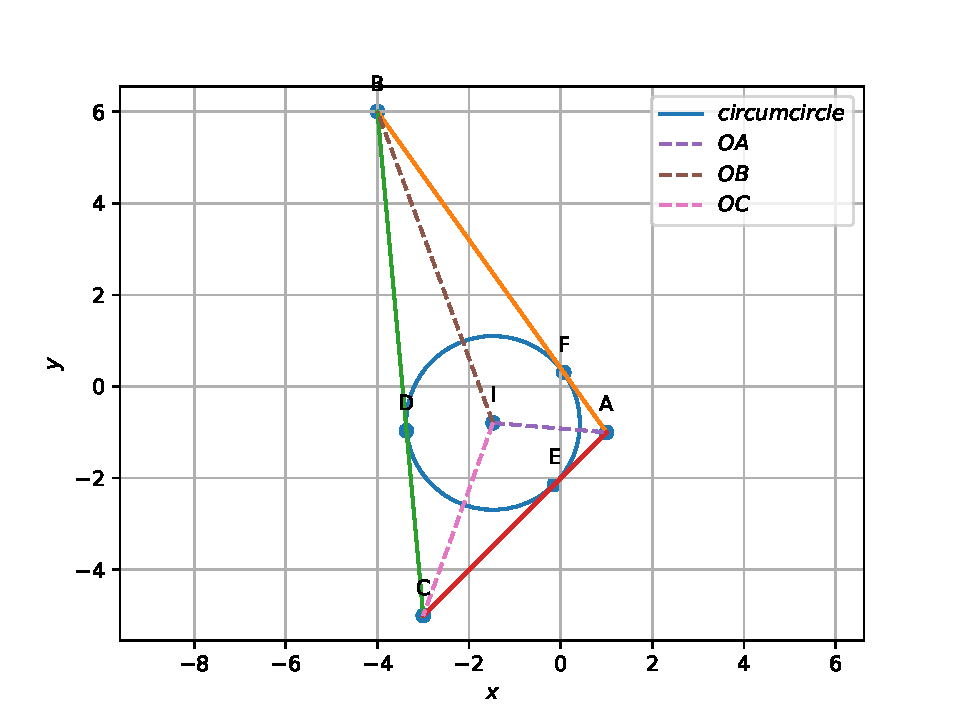
\includegraphics[width=\columnwidth]{figs/triangle/ang-bisect.pdf}
	\caption{Incircle of $\triangle ABC$}
	\label{fig:incircle}
\end{figure}
\iffalse
Considering
\begin{align}
	BC: \quad \vec{n} ^\top \vec{x} &= c, 
\end{align}
the distance from $\vec{I}$ to $BC$ is 
\begin{align}
\frac{\abs{\vec{n}^\top \vec{I} - c}}{\norm{\vec{n}}} 
\end{align}
\fi


	\item Using 
    \eqref{eq:app-angle2d}
verify that 
		\begin{align}
			\angle BAI = \angle CAI.
		\end{align}
		$AI$ is the bisector of $\angle A$.  
	\item Verify that $BI, CI$ are also the angle bisectors of $\triangle ABC$.
All codes for this section are available at
\begin{lstlisting}
	codes/triangle/ang-bisect.py
\end{lstlisting}

\end{enumerate}

\subsection{Eigenvalues and Eigenvectors}
\begin{enumerate}[label=\thesubsection.\arabic*.,ref=\thesubsection.\theenumi]
\item 
	 The equation of a circle is given by 
	\label{prop:circ-eq}
\begin{align}
	\norm{\vec{x}}^2 + 2 \vec{u}^{\top}\vec{x} + f = 0
	\label{eq:circ-eq}
\end{align}
for
		\begin{align}
			 \label{eq:conic_quad_form-params}
	 \vec{u}=-\vec{O}, f = \norm{\vec{O}}-r^2,
		\end{align}
		$\vec{O}$ being the incentre and $r$ the inradius.  
\item Compute 
\begin{align}
	\label{eq:incircle-disc-Sigma}
\vec{\Sigma} = 
\brak{\vec{V}\vec{h}+\vec{u}}
	  \brak{\vec{V}\vec{h}+\vec{u}}^{\top}
   -
	  {g}\brak{\vec{h}}\vec{V}
\end{align}
for $\vec{h}=\vec{A}$.
\item Find the roots of the equation
\begin{align}
	\mydet{\lambda \vec{I}-\vec{\Sigma}} = 0
\end{align}
These are known as the eigenvalues of $\vec{\Sigma}$.
\item Find $\vec{p}$  such that 
\begin{align}
	\vec{\Sigma}\vec{p}
	=\lambda\vec{p}
\end{align}
using row reduction.  These are known as the eigenvectors of $\Sigma$.
\item Define
    \begin{align}
      \label{eq:conic_parmas_eig_def-D}
      \vec{D} &= \myvec{\lambda_1 & 0\\ 0 & \lambda_2}, 
      \\
	    \vec{P} &= \myvec{\frac{\vec{p}_1}{\norm{\vec{p}_1}} & \frac{\vec{p}_2}{\norm{\vec{p}_2}}}
      \label{eq:eigevecP}
    \end{align}
    \item Verify that
  \begin{align}
\vec{P}^{\top}=\vec{P}^{-1}.
  \label{eq:orth-mat}
  \end{align}
  $\vec{P}$ is defined to be an orthogonal matrix.
\item Verify that
    \begin{align}
      \label{eq:conic_parmas_eig_def}
      \vec{P}^{\top}\vec{\Sigma}\vec{P} &= \vec{D},
    \end{align} 
		This is known as the spectral (eigenvalue ) decomposition of a symmetric matrix 

\item
	The direction vectors of the tangents from a point 
$\vec{h}$ to the circle in \eqref{eq:conic_quad_form} are given by  
\begin{align}
  \vec{m}&= \vec{P}\myvec{\sqrt{\abs{\lambda_2}} \\[2mm]  \pm \sqrt{\abs{\lambda_1}}}
	  \label{eq:h-tangents-cond-mPlam}
\end{align}
\item The points of contact of the pair 
of tangents 
to the circle in \eqref{eq:conic_quad_form} 
	from 
	a point $\vec{h}$ 
	are given by 
  \begin{align}
  \label{eq:line_dir_pt-lam}
	  \vec{x}  = \vec{h} + \mu \vec{m}
  \end{align}
  where 
  \begin{align}
  \label{eq:line_dir_pt-lam-mu}
	  \mu = -\frac{\vec{m}^{\top}\brak{\vec{V}\vec{h}+\vec{u}}}{\vec{m}^{\top}\vec{V}\vec{m} }
  \end{align}
	for $\vec{m}$ in 
	  \eqref{eq:h-tangents-cond-mPlam}.
  Compute the points of contact. You should get the same points that you obtained in the previous section. 

All codes for this section are available at
\begin{lstlisting}
	codes/triangle/tangpair.py
\end{lstlisting}
\end{enumerate}

\section{Matrices}
\numberwithin{equation}{section}
The matrix of the veritices of the triangle is defined as
		\begin{align}
			\vec{P} = \myvec{\vec{A} & \vec{B} &\vec{C}}
		\end{align}
		\subsection{Vectors}
\begin{enumerate}[label=\thesection.\arabic*.,ref=\thesubsection.\theenumi]
\numberwithin{equation}{enumi}
\item Obtain the direction matrix of the sides of $\triangle ABC$
	defined as 
		\begin{align}
		\vec{M} = 	\myvec{\vec{A}-\vec{B} & \vec{B}-\vec{C} & \vec{C}-\vec{A}}
		\end{align}
	\\
		\solution 

		\begin{align}
			\vec{M} &= \myvec{\vec{A}-\vec{B} & \vec{B}-\vec{C} & \vec{C}-\vec{A}}
			\\
			&= 
			\myvec{\vec{A} & \vec{B} &\vec{C}}
			\myvec{1 & 0 & -1 \\ -1 & 1 & 0 \\ 0 & -1 & 1}
		\end{align}
		where the second matrix above 
		is known as a {\em circulant} matrix.  Note that the 2nd and 3rd row of the above matrix are circular shifts of the 1st row.
	\item Obtain the normal matrix  of the sides of $\triangle ABC$
		\\
		\solution Considering the roation matrix
		\begin{align}
			\vec{R}  = \myvec{0 & -1 \\ 1 & 0},
		\end{align}
		the normal matrix is obtained as
		\begin{align}
			\vec{N} = \vec{R}\vec{M} 
		\end{align}

	\item Obtain $a, b, c$.
		\\
		\solution The sides vector is obtained as
		\begin{align}
			\vec{d} = \sqrt{\text{diag}(\vec{M}^{\top}\vec{M})}
		\end{align}
	\item Obtain the constant terms in the equations of the sides of the triangle. 
		\\
		\solution The constants for the lines can be expressed in vector form as
		\begin{align}
			\vec{c} = \text{diag}\cbrak{\brak{\vec{N}^{\top}\vec{P}}} 
		\end{align}
\end{enumerate}
		\subsection{Median}
\begin{enumerate}[label=\thesubsection.\arabic*.,ref=\thesubsection.\theenumi]
\numberwithin{equation}{enumi}
\item Obtain the mid point matrix for the sides of the triangle
	\\
		\solution
		\begin{align}
			\myvec{\vec{D} & \vec{E} &\vec{F}} &= \frac{1}{2}\myvec{\vec{A} & \vec{B} &\vec{C}}
			\myvec{0 & 1 & 1 \\ 1 & 0 & 1 \\ 1 & 1 & 0}
		\end{align}
	\item Obtain the median direction matrix.
\\
\solution The median direction matrix is given by 
		\begin{align}
			\vec{M}_1 &= \myvec{\vec{A}-\vec{D} & \vec{B}-\vec{E} & \vec{C}-\vec{F}}
			\\
			&= 
			  \myvec{
				  \vec{A}-\frac{\vec{B}+\vec{C}}{2} &
			  \vec{B}-\frac{\vec{C}+\vec{A}}{2} &
			  \vec{C}-\frac{\vec{A}+\vec{B}}{2}} 
			  \\
			  &= \myvec{\vec{A} & \vec{B} &\vec{C}}
			  \myvec{
				  1 & -\frac{1}{2} & -\frac{1}{2}
				  \\
				  -\frac{1}{2} & 1 & -\frac{1}{2}
				  \\
				  -\frac{1}{2} & -\frac{1}{2} & 1
				  }
		\end{align}
	\item Obtain the median normal matrix.
	\item Obtian the median equation constants.
	\item Obtain the centroid by finding the intersection of the medians.

\end{enumerate}
		\subsection{Altitude}
\begin{enumerate}[label=\thesubsection.\arabic*.,ref=\thesubsection.\theenumi]
\numberwithin{equation}{enumi}
\item Find the normal matrix for the altitudes
	\\
		\solution  The desired matrix is 
\begin{align}
	\vec{M}_2 &= 	\myvec{\vec{B}-\vec{C} & \vec{C}-\vec{A} & \vec{A}-\vec{B} }
	\\
	&= 
	\myvec{\vec{A} & \vec{B} &\vec{C}}
			\myvec{ 0 & -1 & 1 \\ 1 & 0 & -1 \\ -1 & 1 & 0}
		\end{align}

	\item Find the constants vector for the altitudes.
		\\
		\solution The desired vector is 
		\begin{align}
			\vec{c}_2 = \text{diag}\cbrak{\brak{\vec{M}^{\top}\vec{P}}} 
		\end{align}
\end{enumerate}
		\subsection{Perpendicular Bisector}
\begin{enumerate}[label=\thesubsection.\arabic*.,ref=\thesubsection.\theenumi]
\numberwithin{equation}{enumi}
\item Find the normal matrix for the perpendicular bisectors
	\\
	\solution The normal matrix is $\vec{M}_2$
\item Find the constants vector for the perpendicular bisectors.
		\\
		\solution The desired vector is 
		\begin{align}
			\vec{c}_3 = \text{diag}\cbrak{\vec{M}_2^{\top}\myvec{\vec{D} & \vec{E} &\vec{F}}}
		\end{align}

\end{enumerate}
		\subsection{Angle Bisector}
\begin{enumerate}[label=\thesubsection.\arabic*.,ref=\thesubsection.\theenumi]
\numberwithin{equation}{enumi}
\item Find the points of contact.
	\\
		\solution The points of contact are given by 
		\begin{align}
			\myvec{			
						\frac{m\vec{C}+n\vec{B}}{m+n}
			&
			\frac{n\vec{A}+p\vec{C}}{n+p}
			&
						\frac{p\vec{B}+m\vec{A}}{p+m}
			}
			= 	\myvec{\vec{A} & \vec{B} &\vec{C}}
			\myvec{
				0 &			\frac{n}{b} & \frac{m}{c}  
				\\
			 \frac{n}{a}& 0 & \frac{p}{c} 
				\\
			\frac{m}{a}	&		\frac{p}{b} & 0  
			}
		\end{align}
All codes for this section are available at
\begin{lstlisting}
	codes/triangle/mat-alg.py
\end{lstlisting}
\end{enumerate}



\appendices
\section{Points on a Line}
\begin{enumerate}[label=\thesection.\arabic*.,ref=\thesection.\theenumi]
\numberwithin{equation}{enumi}
\item The equation of a line is given by 
\begin{align}
			\label{eq:line-school}
	y &= mx + c
	\\
	\implies \myvec{x \\ y} &= \myvec{x \\ 
	 mx + c} =\myvec{0 \\ c} + x\myvec{1 \\ m}
\end{align}
			yielding \eqref{eq:geo-param}.
\item 			\eqref{eq:line-school} can also be expressed as
\begin{align}
	y - mx &= c 
	\\
	\implies \myvec{-m & 1}\myvec{x \\ y} &= c
\end{align}
			yielding \eqref{eq:geo-normal}.
  \item From \eqref{eq:geo-param}, 
	  if $\vec{A},\vec{D}$ and $\vec{C}$ are on the same line,
		\label{prop:lin-dep}
\begin{align}
			\vec{D}=\vec{A}+q\vec{m} 
			\\ 
			\vec{C}=\vec{D}+p\vec{m} \\
			\label{eq:collinear} 
			\implies 	p\brak{\vec{D}-\vec{A}} 
			+ q\brak{\vec{D}-\vec{C}} = 0, \quad p, q \ne 0 \\ 
			\implies \vec{D} = \frac{p\vec{A}+q\vec{C}}{p+q} 
			\end{align} 
			yielding \eqref{eq:section_formula} upon substituting \begin{align} k = \frac{p}{q}. \end{align} 
			$\brak{\vec{D}-\vec{A}}, \brak{\vec{D}-\vec{C}}$ 
		are then said to be {\em linearly dependent}.
	\item If $\vec{A}, \vec{B}, \vec{C}$ are collinear,  from \eqref{eq:geo-normal}, \begin{align}
	 \vec{n}^{\top}\vec{A} &=  c 
	 \\
	 \vec{n}^{\top}\vec{B} &=  c 
	 \\
	 \vec{n}^{\top}\vec{C} &=  c 
\end{align}
which can be expressed as 
\begin{align}
	\myvec{ \vec{A} & \vec{B} & \vec{C}}^{\top}\vec{n} = c\myvec{1 \\ 1 \\ 1}
	\\
	\implies 
	\myvec{ 1 & 1 &1 \\ \vec{A} & \vec{B} & \vec{C}}^{\top}\myvec{\vec{n} \\ -c} &= \vec{0}
\end{align}
yielding
			\eqref{eq:line-rank}.  Rank is defined to be the number of linearly indpendent rows or columns of a matrix.

  \iffalse
  \item Consequently, points $\vec{A},\vec{B}$ and $\vec{C}$ form a triangle  if 
	  \label{prop:two-tri-indep}
  \begin{align}
	  p\brak{\vec{A}- \vec{B}} +q\brak{\vec{C} -\vec{B}} 
	  \\
	  =\brak{p+q}\vec{B}- p\vec{A} -q\vec{C} = 0
	  \\
	  \implies p=0, q=0
	  \label{eq:two-tri-indep}
  \end{align}
  \item In 
	\figref{fig:tri_med_isect}	
	\begin{align}
	AF = BF, \,
	AE = BE, 
	\end{align}
	and the medians $BE$ and $CF$ meet at $\vec{G}$.
	Show that 
%	Using Fig. \ref{ch2_median_ratio_val}, 
	\begin{align}
\label{eq:tri_med_centroid_ratio}
	\frac{GB}{GE} = \frac{GC}{GF} = 2
	\end{align}
%
\begin{figure}[!ht]
	\begin{center}
		\resizebox{\columnwidth}{!}{%Code by GVV Sharma
%July 8, 2023
%released under GNU GPL
%Drawing the medians

\begin{tikzpicture}
[scale=2,>=stealth,point/.style={draw,circle,fill = black,inner sep=0.5pt},]

%Triangle sides
\def\a{5}
\def\b{6}
\def\c{4}
 
%Coordinates of A
\def\p{2.25}
\def\q{{sqrt(\c^2-\p^2)}}

%Labeling points
\node (A) at (\p,\q)[point,label=above right:$A$] {};
\node (B) at (0, 0)[point,label=below left:$B$] {};
\node (C) at (\a, 0)[point,label=below right:$C$] {};

%Foot of median

%\node (D) at ($(B)!0.5!(C)$)[point,label=below:$D$] {};
\node (E) at ($(A)!0.5!(C)$)[point,label=right:$E$] {};
\node (F) at ($(B)!0.5!(A)$)[point,label=left:$F$] {};

%Drawing triangle ABC
\draw (A) -- node[] {} (B) -- node[below, yshift=-5mm] {$\textrm{a}$} (C) -- node[] {} (A);

%Drawing medians AD, BE and CF
\draw (B) -- (E);
\draw (C) -- (F);
%\draw (A) -- (D);

%Drawing EF
%\draw [dashed] (E) -- (F);

%Centroid
\node (G) at ($(B)!0.67!(E)$)[label={[shift={(0.8,-0.5)}]$G$}] {};

%Labeling sides
\node [right] at ($(A)!0.5!(E)$) {$\frac{b}{2}$};
\node [right] at ($(C)!0.5!(E)$) {$\frac{b}{2}$};
\node [left] at ($(B)!0.5!(F)$) {$\frac{c}{2}$};
\node [left] at ($(A)!0.5!(F)$) {$\frac{c}{2}$};
\node [below] at ($(E)!0.5!(G)$) {$1$};
\node [below] at ($(B)!0.5!(G)$) {$k_1$};
\node [below] at ($(F)!0.5!(G)$) {$1$};
\node [below] at ($(C)!0.5!(G)$) {$k_2$};
\iffalse
\node [above right] at ($(F)!0.5!(E)$) {$P$};
\fi

%\node (G) at ($(B)!0.67!(E)$)[label={[shift={(-0.8,-0.5)}]$G_1$}] {};

%
\end{tikzpicture}

}
	\end{center}
	\caption{$k_1=k_2=2$.}
	\label{fig:tri_med_isect}	
\end{figure}
\solution From 
	  \eqref{eq:section_formula},
  \begin{align}
	  \label{eq:section_formula-G}
\vec{G} = 
	   \frac{k_1\vec{E}+ \vec{B}}{k_1+1}
	  &= \frac{k_2\vec{F}+ \vec{C}}{k_2+1}
	  \\
	  \implies 
	   \frac{k_1\brak{\frac{\vec{A}+\vec{C}}{2}}+ \vec{B}}{k_1+1}
	  &= \frac{k_2\brak{\frac{\vec{A}+\vec{B}}{2}}+ \vec{C}}{k_2+1}
  \end{align}
\begin{multline}
	  \implies 
	\brak{k_2+1}   \cbrak{k_1\brak{{\vec{A}+\vec{C}}}+ 2\vec{B}}
	  \\= \brak{k_1+1}\cbrak{k_2\brak{{\vec{A}+\vec{B}}}+ 2\vec{C}}
\end{multline}
  which can be expressed as
  \begin{align}
	  \cbrak{2 + k_2- k_1k_2 }\vec{B}-\brak{k_2-k_1}\vec{A}  - \cbrak{k_1 +2 - k_1k_2}\vec{C}
	  =0
  \end{align}
  and is of the form
	  \eqref{eq:two-tri-indep}
	  with 
  \begin{align}
	  p = {k_2-k_1}, q = {k_1 +2 - k_1k_2}.
  \end{align}
  Thus, from 
	  \eqref{eq:two-tri-indep}
  \begin{align}
\label{eq:tri_med_centroid_ratio-1}
	  k_2-k_1 &= 0,
	  \\
	  k_1 +2 - k_1k_2 &=0
\label{eq:tri_med_centroid_ratio-2}
  \end{align}
  Thus, from 
\eqref{eq:tri_med_centroid_ratio-2}
  \begin{align}
	  k_1=k_2
  \end{align}
  and substituting the above in 
\eqref{eq:tri_med_centroid_ratio-2} results in the quadratic
  \begin{align}
	  k_1^2 - k_1-2 &=0
	  \\
	  \implies 
	  \brak{k_1-2}\brak{k_1+1} &=0
  \end{align}
  admitting $k_1=k_2=2$ as the only possible solution.
  \item Substituting $k_1 =2 $ in 
	  \eqref{eq:section_formula-G}
  \begin{align}
	  \vec{G}=\frac{\vec{A}+\vec{B} + \vec{C}}{3}
	  \label{eq:centroid-G}
  \end{align}
\item 
In	\figref{fig:tri_med_meet},	
$AG$ is extended to join $BC$ at $\vec{D}$.  Show that $AD$ is also a median.
\begin{figure}[!ht]
	\begin{center}
		\resizebox{\columnwidth}{!}{%Code by GVV Sharma
%December 10, 2019
%released under GNU GPL
%Drawing the median

\begin{tikzpicture}
[scale=2,>=stealth,point/.style={draw,circle,fill = black,inner sep=0.5pt},]

%Triangle sides
\def\a{5}
\def\b{6}
\def\c{4}
 
%Coordinates of A
\def\p{2.25}
\def\q{{sqrt(\c^2-\p^2)}}

%Labeling points
\node (A) at (\p,\q)[point,label=above right:$A$] {};
\node (B) at (0, 0)[point,label=below left:$B$] {};
\node (C) at (\a, 0)[point,label=below right:$C$] {};

%Foot of median

\node (D) at ($(B)!0.5!(C)$)[point,label=below:$D$] {};
\node (E) at ($(A)!0.5!(C)$)[point,label=right:$E$] {};
\node (F) at ($(B)!0.5!(A)$)[point,label=left:$F$] {};

%Drawing triangle ABC
\draw (A) -- node[] {} (B) -- node[below, yshift=-5mm] {$\textrm{a}$} (C) -- node[] {} (A);

%Drawing medians AD, BE and CF
\draw (B) -- (E);
\draw (C) -- (F);
\draw (A) -- (D);

%Drawing EF
\draw [dashed] (E) -- (F);

%Centroid
\node (G) at ($(B)!0.67!(E)$)[label={[shift={(0.8,-0.5)}]$G$}] {};

%Labeling sides
\node [right] at ($(A)!0.5!(E)$) {$\frac{b}{2}$};
\node [right] at ($(C)!0.5!(E)$) {$\frac{b}{2}$};
\node [left] at ($(B)!0.5!(F)$) {$\frac{c}{2}$};
\node [left] at ($(A)!0.5!(F)$) {$\frac{c}{2}$};
\node [below] at ($(E)!0.5!(G)$) {$p$};
\node [below] at ($(B)!0.5!(G)$) {$2p$};
\node [above right] at ($(F)!0.5!(E)$) {$P$};

%\node (G) at ($(B)!0.67!(E)$)[label={[shift={(-0.8,-0.5)}]$G_1$}] {};

%
\end{tikzpicture}

}
	\end{center}
	\caption{$k_3 = 2, k_4 =1$}
	\label{fig:tri_med_meet}	
\end{figure}
	\\
	\solution Considering the ratios in 
	\figref{fig:tri_med_meet},	
  \begin{align}
\vec{G} = 
	  \frac{k_3\vec{D}+\vec{A} }{k_3+1} 
	  \\
	\vec{D}  =\frac{k_4\vec{C}+\vec{B} }{k_4+1} 
  \end{align}
  Substituting from 
	  \eqref{eq:centroid-G}
	  in the above, 
  \begin{align}
	  \brak{k_3+1}\brak{\frac{\vec{A}+\vec{B} + \vec{C}}{3}}
 = 
	  {k_3\brak{\frac{k_4\vec{C}+\vec{B} }{k_4+1}} +\vec{A} } 
  \end{align}
\begin{multline}
	  \implies \brak{k_3+1}\brak{k_4+1}\brak{{\vec{A}+\vec{B} + \vec{C}}}
	  \\
 = 
	  {3} \cbrak{ {k_3\brak{{k_4\vec{C}+\vec{B} }} +\brak{k_4+1}\vec{A} }} 
\end{multline}
  which can be expressed as
  \begin{multline}
	  \brak{k_3k_4+k_3-2k_4-2}\vec{A}
	  \\
	-  \brak{-k_3k_4-k_4+2k_3-1}\vec{B}
	  \\
	  - \brak{-k_3-k_4 - 1 
+2k_3k_4} \vec{C} = \vec{0}
  \end{multline}
  Comparing the above with 
	  \eqref{eq:two-tri-indep},
  \begin{align}
	  p = {-k_3k_4-k_4+2k_3-1}, q = {-k_3-k_4 - 1 
+2k_3k_4}
  \end{align}
  yielding 
  \begin{align}
	  \label{eq:centroid-G-meet-1}
	   {-k_3k_4-k_4+2k_3-1} = 0
	   \\ {-k_3-k_4 - 1 
+2k_3k_4} = 0
	  \label{eq:centroid-G-meet-2}
  \end{align}
  Subtracting 
	  \eqref{eq:centroid-G-meet-1}
	  from
	  \eqref{eq:centroid-G-meet-2},
  \begin{align}
	  3k_3\brak{k_4-1} &= 0
	  \\
	  \implies k_4&=1
  \end{align}
  which upon substituting in 
	  \eqref{eq:centroid-G-meet-1}
	  yields
  \begin{align}
	  k_3 = 2
  \end{align}
  \fi
	  \end{enumerate}

\section{Tangents to a Circle}
\numberwithin{equation}{section}
The equation of the {\em incircle} is given by 
		\begin{align}
			\label{eq:incircle}
			\norm{\vec{x}-\vec{O}}^2 = r^2
		\end{align}
		which can be expressed as 
			 \eqref{eq:conic_quad_form}
			 using 
			 \eqref{eq:conic_quad_form-params}.
	In \figref{fig:incircle}, 
Let 
  \eqref{eq:line_dir_pt-lam}
  be the equation of $AB$.  Then, the intersection of 
  \eqref{eq:line_dir_pt-lam}
  and 
			 \eqref{eq:conic_quad_form}
			 can be expressed as 
\begin{align}
\brak{\vec{h} + \mu{\vec{m}}}^{\top}
\vec{V}
\brak{\vec{h} + \mu{\vec{m}}}
			+2\vec{u}^{\top}\brak{\vec{h} + \mu{\vec{m}}}+f &= 0
			\\
\implies \mu^2\vec{m}^{\top} \vec{V}\vec{m} + 2\mu \vec{m}^{\top}\brak{\vec{V}\vec{h}+\vec{u}}+g\brak{\vec{h}} &= 0 
	\label{eq:incircle-quad}
\end{align}
For 	\eqref{eq:incircle-quad} to have exactly one root, the discriminant
\begin{align}
 \cbrak{\vec{m}^{\top}\brak{\vec{V}\vec{h}+\vec{u}}}^2 -g\brak{\vec{h}}\vec{m}^{\top} \vec{V}\vec{m}  &= 0 
	\label{eq:incircle-disc}
\end{align}
and 
  \eqref{eq:line_dir_pt-lam-mu}
  is obtained.
	\eqref{eq:incircle-disc}
	can be expressed as
\begin{align}
\vec{m}^{\top}\brak{\vec{V}\vec{h}+\vec{u}}^{\top}\brak{\vec{V}\vec{h}+\vec{u}}\vec{m}-g\brak{\vec{h}}\vec{m}^{\top} \vec{V}\vec{m}  &= 0 
\\
\implies \vec{m}^{\top}\vec{\Sigma}\vec{m} &= 0
	\label{eq:incircle-disc-Sigma-new}
\end{align}
for $\vec{\Sigma}$ defined in 
	\eqref{eq:incircle-disc-Sigma-new}.
      Substituting \eqref{eq:conic_parmas_eig_def}
	in \eqref{eq:incircle-disc-Sigma-new},
\begin{align}
\vec{m}^{\top}\vec{P}\vec{D}\vec{P}^{\top}\vec{m} &= 0
\\
\implies 
\vec{v}^{\top}\vec{D}\vec{v} &= 0
	\label{eq:incircle-disc-v}
\end{align}
where 
\begin{align}
	\label{eq:incircle-disc-v-lam-P}
\vec{v} = \vec{P}^{\top}\vec{m}
\end{align}
	\eqref{eq:incircle-disc-v}
	can be expressed as 
\begin{align}
\lambda_1 v_1^2
-\lambda_2 v_2^2 &= 0
\\
\implies \vec{v} = \myvec{\sqrt{\abs{\lambda_2}} \\[2mm]  \pm \sqrt{\abs{\lambda_1}}}
	\label{eq:incircle-disc-v-lam}
\end{align}
after some algebra.
From 
	\eqref{eq:incircle-disc-v-lam}
	and
	\eqref{eq:incircle-disc-v-lam-P}
	we obtain 
	  \eqref{eq:h-tangents-cond-mPlam}.



\iffalse
\section{Baudhayana Theorem}
\subsection{The Right Angled Triangle}
A right angled triangle looks like Fig. \ref{fig:tri_right_angle}.
\begin{figure}[!ht]
\centering
\resizebox{\columnwidth}{!}{%Code by GVV Sharma
%December 6, 2019
%released under GNU GPL
%Drawing a right angled triangle

\begin{tikzpicture}[scale=2]

%Triangle sides
\def\a{4}
\def\c{3}

%Marking coordiantes
\coordinate [label=above:$A$] (A) at (0,\c);
\coordinate [label=left:$B$] (B) at (0,0);
\coordinate [label=right:$C$] (C) at (\a,0);

%Drawing triangle ABC
\draw (A) -- node[left] {$\textrm{c}$} (B) -- node[below] {$\textrm{a}$} (C) -- node[above,,xshift=2mm] {$\textrm{b}$} (A);

%Drawing and marking angles
\tkzMarkAngle[fill=orange!40,size=0.5cm,mark=](A,C,B)
\tkzMarkRightAngle[fill=blue!20,size=.3](A,B,C)
\tkzLabelAngle[pos=0.65](A,C,B){$\theta$}
\end{tikzpicture}
}
\caption{Right Angled Triangle}
\label{fig:tri_right_angle}	
\end{figure}
with angles $\angle A,\angle B$ and $\angle C$ and sides $a, b$ and $c$.  The unique feature of this triangle is $\angle B$ which is defined to be $90\degree$.
%\renewcommand{\theequation}{\theenumi}
\begin{enumerate}[label=\thesection.\arabic*.,ref=\thesection.\theenumi]
\numberwithin{equation}{enumi}
\item
	For simplicity, let the greek letter $\theta = \angle C$.  We have the following definitions.
\begin{equation}
\label{eq:tri_trig_defs}
\begin{matrix}
	\sin \theta = \frac{c}{b} & 	\cos \theta = \frac{a}{b} \\
	\tan \theta = \frac{c}{a} & \cot \theta = \frac{1}{\tan \theta} \\
	\csc \theta = \frac{1}{\sin \theta} & \sec \theta = \frac{1}{\cos \theta}
	\end{matrix}
\end{equation}
%
\item  Show that
	\begin{equation}
	\cos \theta = \sin \brak{90\degree - \theta}
	\label{eq:tri_baudh_comp}	
	\end{equation}
\solution From \eqref{eq:tri_trig_defs},
%
\begin{align}
\label{eq:tri_90-ang}
\cos \angle BAC = \cos \alpha =	\cos \brak{90\degree-\theta} = \frac{c}{b} 
%\\
= \sin \angle ABC = \sin \theta
\end{align}
\iffalse
\item Draw Fig. \ref{fig:tri_right_angle} for $a = 4, c =3$.
\label{const:tri_right_angle}
%
\\
\solution The vertices of $\triangle ABC$ are 
\begin{align}
\vec{A} = \myvec{0\\c} = \myvec{0\\3}, \vec{B} = \myvec{0\\0}, \vec{C} = \myvec{a\\0}=\myvec{4\\0}
\end{align}
%
The python code for  Fig. \ref{fig:tri_right_angle} is
\begin{lstlisting}
codes/triangle/tri_right_angle.py
\end{lstlisting}
%
and the equivalent latex-tikz code is
%
\begin{lstlisting}
figs/triangle/tri_right_angle.tex
\end{lstlisting}
%
The above latex code can be compiled as a standalone document as
%
\begin{lstlisting}
figs/triangle/tri_right_angle_alone.tex
\end{lstlisting}
%
\item Draw Fig. \ref{fig:tri_polar} for $a = 4, c =3$.
\label{const:tri_polar}
%
\\
\solution The vertices of $\triangle ABC$ are 
\begin{align}
\vec{A} = \myvec{a\\c} = \myvec{4\\3}, \vec{B} = \myvec{a\\0}  = \myvec{4\\0}, \vec{C} = \myvec{0\\0}.
\end{align}
%
The python code for  Fig. \ref{fig:tri_polar} is
\begin{lstlisting}
codes/triangle/tri_polar.py
\end{lstlisting}
%
and the equivalent latex-tikz code is
%
\begin{lstlisting}
figs/triangle/tri_polar.tex
\end{lstlisting}
\begin{figure}[!ht]
\centering
\resizebox{\columnwidth}{!}{%Code by GVV Sharma
%December 6, 2019
%released under GNU GPL
%Drawing a right angled triangle

\begin{tikzpicture}[scale=2]

%Triangle sides
\def\a{4}
\def\c{3}

%Marking coordiantes
\coordinate [label=above:$A$] (A) at (\a,\c);
\coordinate [label=below:$B$] (B) at (\a,0);
\coordinate [label=left:$C$] (C) at (0,0);

%Drawing triangle ABC
\draw (A) -- node[left] {$\textrm{c}$} (B) -- node[below] {$\textrm{a}$} (C) -- node[above left,xshift=2mm] {$\textrm{b}$} (A);

%Drawing and marking angles
\tkzMarkAngle[fill=orange!40,size=0.5cm,mark=](B,C,A)
\tkzMarkRightAngle[fill=blue!20,size=.3](A,B,C)
\tkzLabelAngle[pos=0.65](A,C,B){$\theta$}
\end{tikzpicture}
}
\caption{Right Angled Triangle}
\label{fig:tri_polar}	
\end{figure}
%
\item The vertex  $\vec{A}$ can also be expressed  in {\em polar coordinate form} as
\label{prob:tri_polar}
%
\begin{align}
\vec{A} = \myvec{b\cos \theta\\ b \sin \theta} 
\end{align}
%
\fi

\end{enumerate}


\subsection{Sum of Angles}
Refer to \figref{fig:tri_sum_angle}.
%\renewcommand{\theequation}{\theenumi}
\begin{enumerate}[label=\thesection.\arabic*.,ref=\thesection.\theenumi]
\numberwithin{equation}{enumi}
\item 	In Fig. \ref{fig:tri_sum_angle}, the sum of all the angles on the top or bottom side of the straight line $XY$ is $180\degree$.


\begin{figure}[!ht]
	\begin{center}
		\resizebox{\columnwidth}{!}{%Code by GVV Sharma
%December 6, 2019
%released under GNU GPL
%Sum of the angles of a right angled triangle 

\begin{tikzpicture}
[scale=2,>=stealth,point/.style={draw,circle,fill = black,inner sep=0.5pt},]

%Triangle sides
\def\a{4}
\def\c{3}

%Section Ratio
\def\k{1.2}


%Labeling points
\node (A) at (0,\c)[point,label=above right:$A$] {};
\node (B) at (0, 0)[point,label=below left:$B$] {};
\node (C) at (\a, 0)[point,label=below right:$C$] {};

%Translating coordinates
\node (Y) at ($(A) + (1,0)$)[point,label=above right:$Y$] {};
\node (X) at ($(A) - (1,0)$)[point,label=above right:$X$] {};
\node (T) at ($(A) + (0,1)$)[point,label=above right:$T$] {};

%Section formula
\node (V) at ($ (C)!\k!(A) $)[point,label=above right:$V$] {};

%Drawing triangle ABC
\draw (A) -- node[left] {$\textrm{c}$} (B) -- node[below] {$\textrm{a}$} (C) -- node[above,xshift=2mm] {$\textrm{b}$} (A);

%Joining other points
\draw (Y)--(A);
\draw (X)--(A);
\draw (T)--(A);
\draw (V)--(A);

%Drawing and marking angles
\tkzMarkAngle[fill=orange!40,size=0.5cm,mark=](A,C,B)
\tkzMarkAngle[fill=orange!40,size=0.5cm,mark=](V,A,X)
\tkzMarkRightAngle[fill=blue!20,size=.3](A,B,C)
\tkzMarkRightAngle[fill=blue!20,size=.3](B,A,X)
\tkzLabelAngle[pos=0.65](A,C,B){$\theta$}
\tkzLabelAngle[pos=0.65](V,A,X){$\theta$}

\end{tikzpicture}
}
	\end{center}
	\caption{Sum of angles of a triangle}
	\label{fig:tri_sum_angle}	
\end{figure}



\item
In Fig. \ref{fig:tri_sum_angle}, the straight line making an angle of $90\degree$ to the side $AB$ is said to be parallel to the side $BC$. Note there is an angle at $A$ that is equal to $\theta$.  This is one property of parallel lines.  Thus, $\angle YAZ = 90\degree$.


\item
	Show that $\angle VAT = 90\degree - \theta$
		
	\solution Considering the line $XAT$,
	\begin{align}
	\theta + 90\degree + \angle VAT &= 180\degree \\
	\Rightarrow  \angle VAT =  90\degree - \theta
	\end{align}

\item
	\label{prob:tri_compl_angle}
	Show that $\angle BAC = 90\degree - \theta$.
	
	\solution Consider the line $VAB$ and and use the approach in the previous problem.  Note that this implies that $\angle VAT = \angle BAC$.  Such angles are known as vertically opposite angles. 
	 
\item
Sum of the angles of a triangle is equal to $180\degree$.
%
\iffalse
\item Draw Fig. \ref{fig:tri_sum_angle} for $a = 4, c =3$.
%
\\
\solution Problem \ref{const:tri_right_angle} is used to draw $\triangle ABC$.  
		The remaining points are obtained as

\begin{align}
\vec{Y} &= \vec{A} + \myvec{1\\0} = \myvec{1\\3}
\\
\vec{X} &= \vec{A} - \myvec{1\\0} = \myvec{-1\\3}
\\
\vec{T} &= \vec{A} + \myvec{0\\1} = \myvec{0\\4}
\end{align}
%
and 
\begin{align}
\frac{VC}{AC} &= k+1
\\
\label{eq:tri_section_formula}
\implies \vec{A} &= \frac{k\vec{C} + \vec{V}}{k+1}  
\\
\implies \vec{V} &= {\brak{k+1}\vec{A} - k\vec{C}}
\end{align}
%
for $k = 0.2$. \eqref{eq:tri_section_formula} is known as the {\em section formula}.
%
The python code for  Fig. \ref{fig:tri_sum_angle} is
\begin{lstlisting}
codes/triangle/tri_sum_angle.py
\end{lstlisting}
%
and the equivalent latex-tikz code is
%
\begin{lstlisting}
figs/triangle/tri_sum_angle.tex
\end{lstlisting}
\fi
\end{enumerate}

\subsection{Proof of Baudhayana Theorem}
Use Fig. \ref{fig:tri_baudh} for all problems in this section.
\begin{figure}[!ht]
	\begin{center}
		\resizebox{\columnwidth}{!}{%Code by GVV Sharma
%December 7, 2019
%released under GNU GPL
%Proof of Baudhyana Theorem

\begin{tikzpicture}
[scale=2,>=stealth,point/.style={draw,circle,fill = black,inner sep=0.5pt},]

%Triangle sides
\def\a{4}
\def\c{3}
\def\b{sqrt(\a^2+\c^2)}

%Trigonometric ratios
\def\ct{\a/\b}
\def\st{\c/\b}

%perp distance
\def\r{\a*\st}

%Section Ratio
\def\k{1.2}


%Labeling points
\node (A) at (0,\c)[point,label=above right:$A$] {};
\node (B) at (0, 0)[point,label=below left:$B$] {};
\node (C) at (\a, 0)[point,label=below right:$C$] {};

%Foot of perpendicular

\node (D) at ($({\r*\st}, {\r*\ct})$)[point,label=above right:$D$] {};


%Drawing triangle ABC
\draw (A) -- node[left] {$\textrm{c}$} (B) -- node[below] {$\textrm{a}$} (C) -- node[above,xshift=2mm] {$\textrm{b}$} (A);

%Joining BD
\draw (B)--(D);

%Drawing and marking angles
\tkzMarkAngle[fill=orange!40,size=0.5cm,mark=](A,C,B)
\tkzMarkAngle[fill=orange!40,size=0.4cm,mark=](D,B,A)
\tkzMarkAngle[fill=green!40,size=0.5cm,mark=](B,A,C)
\tkzMarkAngle[fill=green!40,size=0.5cm,mark=](C,B,D)
\tkzMarkRightAngle[fill=blue!20,size=.2](A,B,C)
\tkzMarkRightAngle[fill=blue!20,size=.2](B,D,A)
\tkzLabelAngle[pos=0.65](A,C,B){$\theta$}
\tkzLabelAngle[pos=0.65](A,B,D){$\theta$}
\tkzLabelAngle[pos=1](B,A,C){\rotatebox{-45}{$\alpha = 90\degree -\theta$}}
\tkzLabelAngle[pos=0.65](C,B,D){$\alpha$}

\end{tikzpicture}
}
	\end{center}
	\caption{Baudhayana Theorem}
	\label{fig:tri_baudh}	
\end{figure}
\renewcommand{\theequation}{\theenumi}
\begin{enumerate}[label=\thesection.\arabic*.,ref=\thesection.\theenumi]
\numberwithin{equation}{enumi}

%
\item
Show that 
%
\begin{equation}
\label{ch1_budh_basic}
b = a \cos \theta + c \sin \theta
\end{equation}
%
\solution We observe that
%
\begin{align}
BD &= a \cos \theta \\
AD &= c \cos\alpha = c \sin \theta \quad \brak{\text{From} \quad \eqref{eq:tri_90-ang}
}
\end{align}
%
Thus,
\begin{equation}
BD + AD = b = a \cos \theta + c \sin \theta
\end{equation}
\item
From \eqref{ch1_budh_basic}, show that
%
\begin{equation}
%
\label{eq:tri_sin_cos_id}
\sin ^2 \theta + \cos ^2 \theta = 1
\end{equation}
%
\solution Dividing both sides of \eqref{ch1_budh_basic} by $b$, 
\begin{align}
1 &= \frac{a}{b}\cos\theta + \frac{c}{b}\sin\theta\\
\Rightarrow &\sin ^2 \theta + \cos ^2 \theta = 1 \quad \brak{\text{from} \quad \eqref{eq:tri_trig_defs}}
\end{align}
\item In a right angled triangle, the hypotenuse is the longest side.
\label{them:hyp_largest}
\\
\solution From 
\eqref{eq:tri_sin_cos_id},
\begin{align}
	0 \le \sin \theta, \cos \theta \le 1
\end{align}
Hence, 
\begin{align}
	b \sin \theta \le b \implies  c \le b
\end{align}
Similalry,
\begin{align}
	a \le b
\end{align}

\item
	Using \eqref{ch1_budh_basic}, show that
	\begin{equation}
	\label{eq:tri_baudh}
	b^2 = a^2 + c^2
	\end{equation}
	\eqref{eq:tri_baudh} is known as the Baudhayana theorem.  It is also known as the Pythagoras theorem.
\\
\solution From \eqref{ch1_budh_basic},
\begin{align}
b &= a\frac{a}{b} + c \frac{c}{b} \quad \brak{\text{from} \quad \eqref{eq:tri_trig_defs}}\\
\implies b^2 &= a^2 + c^2
\end{align}
\end{enumerate}
%
\iffalse
\section{Applications}
\begin{enumerate}[label=\thesection.\arabic*.,ref=\thesection.\theenumi]
\numberwithin{equation}{enumi}
\item Show that $c > a, c > b$
%
	\\
\solution From 	\eqref{eq:tri_baudh},
	\begin{align}
	c^2 - a^2 &= b^2
\\
\implies c-a &= \frac{b^2}{c+a} > 0 
\\
\implies c &> a
	\end{align}
%
Similarly, it can be shown that $c > b$.
\iffalse
\item Draw Fig. \ref{fig:tri_baudh} for $a = 4, c =3$.
\label{const:tri_baudh}
%
\\
\solution Problem \ref{const:tri_right_angle} is used to draw $\triangle ABC$.
%
Using Problem \ref{prob:tri_polar},
\begin{align}
\vec{D} &= BD\myvec{\cos \alpha\\  \sin \alpha} 
&= a \sin \theta \myvec{ \sin \theta \\ \cos \theta } 
\label{eq:tri_baudh_foot}
\end{align}
%
Using \eqref{eq:tri_baudh_foot}, the python code for  Fig. \ref{fig:tri_baudh} is
\begin{lstlisting}
codes/triangle/tri_baudh.py
\end{lstlisting}
%
and the equivalent latex-tikz code is
%
\begin{lstlisting}
figs/triangle/tri_baudh.tex
\end{lstlisting}
%
\item Using 	\eqref{eq:tri_baudh}, for $a = 4, c = 3$,
%
\begin{align}
b = \sqrt{a^2+c^2} = \sqrt{4^2+3^2} = 5
\end{align}
%
\item For  point $\vec{D} = \myvec{d_1\\d_2}$, its {\em norm} is defined as
%
\begin{align}
OD = d_1^2+d_2^2 = \norm{\vec{D}} \define \sqrt{\vec{D}^{\top}\vec{D}}, 
\label{eq:tri_norm_def}
\end{align}
%
where 
%
\begin{align}
\label{eq:tri_transpose_def}
 \vec{D}^{\top}  \define \myvec{d_1 & d_2},
\\
\vec{D}^{\top}\vec{D} \define \myvec{d_1 & d_2} \myvec{d_1 \\ d_2} = d_1^2+d_2^2
\end{align}
%
\eqref{eq:tri_transpose_def} is the definition of {\em transpose}. $\vec{D}$ is defined to be a {\em column vector} and $\vec{D}^{\top}$  is the corresponding {\em row vector} representing the same point.

\item Also, it is easy to verify that
%
\begin{align}
\label{eq:tri_norm_dist}
AC \define  \norm{\vec{A}-\vec{C}} =  \norm{\myvec{4\\-3}} = \sqrt{3^2+4^2} = 5
\end{align}
%
This is known as the {\em distance formula}.
\fi
%
\item Prove the distance formula in 
  \eqref{eq:norm2d_dist}
 using the Baudhayana theorem.
%
\item Show that 
\label{them:tri_baudh_orth}
\begin{align}
\label{eq:tri_baudh_orth}
\brak{\vec{A}-\vec{B}}^{\top}\brak{\vec{B}-\vec{C}} = 0
\end{align}
\\
\solution From the Baudhayana theorem,
\begin{align}
a^2+c^2 &= b^2
\\
\implies \norm{\vec{B}-\vec{A}}^2+\norm{\vec{C}-\vec{A}}^2&=\norm{\vec{B}-\vec{C}}^2
\label{eq:tri_baudh_orth_norm}
\end{align}
which, from 
  \eqref{eq:norm2d}
 can be expressed as
\begin{multline}
\brak{\vec{B}-\vec{A}}^{\top}\brak{\vec{B}-\vec{A}}
+
\brak{\vec{C}-\vec{B}}^{\top}\brak{\vec{C}-\vec{B}}
\\
=
\brak{\vec{A}-\vec{C}}^{\top}\brak{\vec{A}-\vec{C}}
\end{multline}
%
Expanding
\begin{multline}
\brak{\vec{B}-\vec{A}}^{\top}\brak{\vec{B}-\vec{A}} 
%\\
= \vec{B}^{\top}\vec{B} - \vec{B}^{\top}\vec{A} - \vec{A}^{\top}\vec{B}+\vec{A}^{\top}\vec{A}
\end{multline}
$\because \vec{A}^{\top}\vec{B} = \vec{B}^{\top}\vec{A}$, the above equation can be expressed as
\begin{align}
\norm{\vec{B}-\vec{A}}^2 = 
\norm{\vec{A}}^2 + \norm{\vec{B}}^2 - 2\vec{A}^{\top}\vec{B}
\end{align}
%
Thus, \eqref{eq:tri_baudh_orth_norm} can be expressed using the above equation as
\begin{multline}
\norm{\vec{A}}^2 + \norm{\vec{B}}^2 - 2\vec{A}^{\top}\vec{B}
%\\
+
\norm{\vec{B}}^2 + \norm{\vec{C}}^2 - 2\vec{B}^{\top}\vec{C}
\\
=
\norm{\vec{A}}^2 + \norm{\vec{C}}^2 - 2\vec{A}^{\top}\vec{C}
\end{multline}
%
which can be simplified to obtain
%
\begin{align}
2\norm{\vec{B}}^2 - 2\vec{B}^{\top}\vec{C}
%\\
- 2\vec{A}^{\top}\vec{B}+ 2\vec{A}^{\top}\vec{C}
=0
\\
\text{or, } \vec{B}^{\top}\brak{\vec{B}-\vec{C}}
-\vec{A}^{\top}\brak{\vec{B}-\vec{C}} = 0
\\
\implies \brak{\vec{B}^{\top}-\vec{A}^{\top}}\brak{\vec{B}-\vec{C}} = 0
\end{align}
yielding \eqref{eq:tri_baudh_orth}.
\end{enumerate}
\fi

\fi


\end{document}


